\documentclass[final,5p,times,twocolumn]{elsarticle}

\usepackage{amsmath,amssymb,amsfonts}
\usepackage{graphicx}
\usepackage{booktabs}
\usepackage{multirow}
\usepackage[table]{xcolor}
\usepackage{array}
\usepackage[ruled,vlined,linesnumbered]{algorithm2e}
\usepackage[hidelinks,pdfencoding=auto]{hyperref}

\definecolor{oursrow}{RGB}{236,244,251}
\renewcommand{\topfraction}{0.92}
\renewcommand{\bottomfraction}{0.85}
\renewcommand{\textfraction}{0.07}
\renewcommand{\floatpagefraction}{0.82}
\renewcommand{\dbltopfraction}{0.92}
\renewcommand{\dblfloatpagefraction}{0.82}
\setcounter{topnumber}{3}
\setcounter{dbltopnumber}{3}
\setcounter{totalnumber}{5}
\journal{Computer Communications}

\begin{document}

\begin{frontmatter}

\title{BorrowedSight: Category-Geometry Token Communication and Visibility Envelopes for Zero-Ego-Observation Cooperative 3D Semantic Occupancy}

\author[scnu]{Yonghao Wu\corref{cor1}}
\ead{yonghaowu369@gmail.com}
\cortext[cor1]{First author and corresponding author.}
\affiliation[scnu]{
  organization={School of Electronic Science and Engineering (School of Microelectronics), South China Normal University},
  city={Foshan},
  state={Guangdong},
  country={China}
}

\begin{abstract}
Connected automated vehicles navigating urban corridors routinely share the road with legacy or sensor-degraded vehicles that retain 6-DoF localization and V2X radios yet possess zero functional onboard perception sensors. Existing cooperative 3D semantic occupancy systems break down in this zero-ego-observation regime because they rely on active ego camera or LiDAR backbones, allocate monolithic shared codebooks that let abundant planar road voxels crowd out dynamic obstacles, and conflate unobserved blind space with verified free space. This paper introduces BorrowedSight, a pure-PyTorch, receiver-centric cooperative 3D semantic occupancy framework engineered strictly for zero-ego-observation V2X links. Neighboring LiDAR-equipped vehicles extract voxel features and six local geometric moments, enforce category-balanced token quotas, and pack every transmitted anchor into a zero-waste 5-byte (40-bit) wire record uniting a 17-bit lossless voxel coordinate, a 4-bit semantic class anchor, two 6-bit geometry-group ResidualSimVQ codes across three specialized codebooks (Things, Ground, and Vertical Static), and 7-bit confidence. Self-contained 16-token Morton micro-blocks isolate wireless packet drops alongside a fixed 512-byte Zstandard slot carrying an adaptive $50\times 50$ visibility envelope and $25\times 25$ max-height prior at zero extra wire bytes. On the receiver side, Task-Decoupled Visibility Fusion (TDVF) routes dense visibility envelopes exclusively into a late-fusion tri-state refinement branch, eliminating geometric shortcut overfitting in the shared semantic U-Net stem while training with masked Lov\'asz-Softmax, asymmetric blind-zone free-space penalties, and randomized multi-budget exposure. Across 25 disjoint multi-sender real OPV2V and Semantic-OPV2V scenes (2,383 frames, 2--5 CAVs) at exact 0.0\% byte discrepancy, BorrowedSight attains $0.4255 \pm 0.0065$ held-out test mIoU (\textbf{B4-Compact}, 2.34M parameters, 15.22~GFLOPs) and $0.4168 \pm 0.0043$ mIoU with top vehicle IoU ($0.4865 \pm 0.0024$) and lowest blind-zone error (UFE $0.0364 \pm 0.0047$, \textbf{B4-TDVF}, 2.42M parameters, 16.70~GFLOPs) at 32,768~B (2.62~Mbps at 10~Hz), surpassing equal-byte sparse continuous (0.2732), projected continuous (0.3640), and compact 4-byte shared-VQ ($0.4044 \pm 0.0080$) baselines while outperforming published 4-camera ego-equipped VQSOP (0.4154) with zero ego sensors. At half bandwidth (16,384~B), \textbf{B4-TDVF} achieves $0.4067 \pm 0.0093$ mIoU and $0.4861 \pm 0.0053$ vehicle IoU, beating the full-bandwidth 32~KB shared-VQ baseline at half the wireless rate, while multi-budget training reaches 0.3702~mIoU at 8,192~B (0.66~Mbps) and 0.3250 at 4,096~B (0.33~Mbps). Scene-grouped 5-fold cross-validation across all 25 disjoint scenes further confirms statistically significant 10/10 paired fold wins ($p = 0.0023$ at 16~KB, $p = 0.0430$ at 32~KB). Vectorized pure-PyTorch inference runs at 10.57--11.90~ms (84.0--94.6~FPS) for one sender and 34.53--39.19~ms (25.5--29.0~FPS) for four simultaneous senders within 170.5~MB peak VRAM on one RTX~3090, maintaining consistent gains under LISA fog, rain, latency, pose noise, and 50\% micro-block loss. Reproducible code and protocol audits are publicly available at \texttt{https://github.com/WYH302/BorrowedSight}.
\end{abstract}

\begin{highlights}
\item Formalizes strict zero-ego cooperative 3D semantic occupancy over V2X links.
\item Zero-waste 5 B/token packing pairs class embeddings with 2-stage grouped VQ.
\item Task-decoupled 50x50 Zstd visibility envelopes cut UFE without semantic drop.
\item Reaches 0.4255 mIoU (32 KB) and 0.4067 at 16 KB (beats 32 KB shared VQ).
\item Pure-PyTorch pipeline runs at 84-95 FPS (1 sender) and 26-29 FPS (4 senders).
\end{highlights}

\begin{keyword}
Cooperative perception \sep V2X communications \sep 3D semantic occupancy \sep Residual vector quantization \sep Visibility-aware fusion \sep Autonomous vehicles
\end{keyword}

\end{frontmatter}

\section{Introduction}

Mixed-autonomy traffic will define urban roadways for decades. Vehicles equipped with multi-beam LiDAR and onboard compute routinely share congested corridors with lower-cost legacy vehicles or connected vehicles whose cameras and LiDAR units suffer sudden mud, lens icing, dense fog, or hardware failure~\cite{bijelic2020fog,kilic2021lisa,etsi2023cpm}. Whenever an ego vehicle loses local environmental sensing yet retains six-degree-of-freedom (6-DoF) localization and a vehicle-to-everything (V2X) transceiver, neighboring connected automated vehicles (CAVs) become its sole source of spatial awareness. Reconstructing a dense, receiver-centric 3D semantic occupancy grid purely from neighbor transmissions within practical wireless budgets (0.66--2.62~Mbps at 10~Hz) is therefore a core vehicular communication and operational-safety challenge.

Existing cooperative perception systems fail structurally in this zero-ego-observation regime for three coupled reasons. First, feature-fusion architectures such as F-Cooper~\cite{chen2019fcooper}, V2VNet~\cite{wang2020v2vnet}, V2X-ViT~\cite{xu2022v2xvit}, and CoBEVT~\cite{xu2022cobevt}, as well as collaborative 3D occupancy frameworks such as CoHFF~\cite{song2024cohff}, Co3SOP~\cite{wu2025co3sop}, VOGS-CP~\cite{chen2026vogscp}, and VQSOP~\cite{li2026vqsop}, depend on an active ego perception tower that anchors local geometry and free space. Neighbor streams act merely as auxiliary context. Stripped of ego sensors, dense floating-point feature broadcasts saturate V2X links, whereas standardized object-level collective perception messages (ETSI CPM)~\cite{etsi2023cpm} discard road topology, curbs, guardrails, and drivable free corridors.

Second, existing discrete V2X tokenizers suffer semantic-geometric interference under tight packet budgets. Codebook compressors such as CodeFilling~\cite{hu2024codefilling} and shared sparse vector-quantized occupancy models~\cite{li2026vqsop} map all 3D semantic classes into a single monolithic codebook without category quotas. In real LiDAR sweeps, abundant planar road voxels consume an outsized share of wire slots while diverse vertical structures (buildings, poles, vegetation, signs, and vehicles) compete for the same finite prototype pool, degrading minority-class recall and amplifying training variance.

Third, and most critically for downstream planning safety, sparse anchor messaging conflates \textit{unobserved blind volume} with \textit{observed free space}. Transmitting only occupied surface tokens leaves every unreceived voxel in a zero-ego receiver grid geometrically ambiguous: a cell may be empty because a neighbor laser ray traversed it cleanly, or because an occluding truck, heavy fog attenuation, or a dropped wireless block prevented any ray from ever sampling it. Decoders trained under standard empty-versus-occupied supervision paint occluded blind zones as confident free space, creating silent collision hazards.

To resolve all three bottlenecks within one bandwidth-disciplined wire protocol, we present \textbf{BorrowedSight}, a lightweight pure-PyTorch framework for zero-ego-observation cooperative 3D semantic occupancy. Rather than inflating backbone capacity, BorrowedSight redesigns what information enters every wire bit under matched encoder and decoder networks. Each LiDAR-equipped neighbor extracts voxel semantics and six local geometric descriptors, applies category-balanced token quotas that protect dynamic vehicles and vertical structures from road-token crowding, and packs every anchor into a zero-waste \textbf{5-byte (40-bit)} token combining a lossless 17-bit 3D voxel coordinate, a 4-bit semantic class identifier, two 6-bit geometry-group ResidualSimVQ codes (Things, Ground, and Vertical Static)~\cite{zhu2025simvq,fifty2025rotation}, and 7-bit confidence. Because the 4-bit class identifier travels losslessly inside the 40-bit record, adding a shared 208-parameter class embedding $\mathbf{E}_{\mathrm{cls}}$ at the receiver incurs \textit{zero extra wire bits} and eliminates inter-class codebook interference, raising held-out mIoU by over 2 percentage points and slashing cross-seed dispersion while making Stage-2 residual refinement completely free in packet bytes.

Selected anchors are organized into self-contained 16-token Morton micro-blocks so wireless block loss never corrupts surviving blocks, paired with an optional fixed 512-byte Zstandard (Zstd) slot that adaptively compresses a $50\times 50$ ($0.8\,\mathrm{m}$) tri-state visibility envelope plus a $25\times 25$ maximum-height prior derived strictly from neighbor LiDAR ray traversal. On the receiver side, a key architectural insight prevents high-resolution visibility grids from degrading semantic generalization: feeding dense $50\times 50$ occupancy and height maps directly into the shared semantic U-Net stem induces geometric shortcut overfitting that lowers held-out test mIoU by 1.39 points and degrades blind-zone safety. BorrowedSight resolves this conflict via \textbf{Task-Decoupled Visibility Fusion (TDVF)}, isolating backward-warped $\mathrm{SE}(3)$ visibility envelopes inside a lightweight late-fusion tri-state refinement branch while training end-to-end with masked Lov\'asz-Softmax~\cite{berman2018lovasz}, asymmetric unobserved-as-free penalties, and randomized 4--32~KB multi-budget exposure.

The primary contributions of this work are as follows:
\begin{itemize}
\item \textbf{Strict Zero-Ego Cooperative Occupancy Formulation and Audit Suite:} We formalize zero-ego-observation cooperative 3D semantic occupancy, construct causal sender-ray tri-state ground truth separating verified free corridors from unobserved blind volumes, and verify non-leakage through six automated invariants across both synthetic and real OPV2V streams.
\item \textbf{Zero-Waste 5-Byte Category-Geometry Micro-Block Protocol with Adaptive $50\times 50$ Zstd Envelopes:} We engineer an equalized-byte protocol packing lossless 17-bit coordinates, 4-bit semantic anchors, free Stage-2 grouped ResidualSimVQ codes, and 7-bit confidence into exact 40-bit tokens alongside a fixed 512-byte adaptive Zstd slot that fits $50\times 50$ visibility grids across 100\% of all 4,736 real OPV2V sweeps at zero extra wire bytes.
\item \textbf{Task-Decoupled Visibility Fusion (TDVF) and Comprehensive Multi-Scene Validation:} We diagnose geometric shortcut overfitting from early envelope injection and resolve it with late-fusion TDVF (+1.39~mIoU pts and $-20.6\%$ UFE over shared-stem fusion). Across 25 disjoint real OPV2V scenes (2,383 frames, 2--5 CAVs), BorrowedSight achieves $0.4255 \pm 0.0065$ mIoU (\textbf{B4-Compact}) and $0.4168 \pm 0.0043$ mIoU / $0.4865$ vehicle IoU / $0.0364$ UFE (\textbf{B4-TDVF}) at 32~KB---exceeding 4-camera ego-equipped VQSOP (0.4154) with zero ego sensors---beats 32~KB compact shared VQ at half bandwidth (16~KB: $0.4067$), reaches $0.3702$ mIoU at 8~KB (0.66~Mbps), and confirms 10/10 statistically significant wins in 25-scene 5-fold cross-validation ($p = 0.0023$ at 16~KB).
\item \textbf{Real-Time Vectorized Pure-PyTorch Deployment and End-to-End V2X Resilience:} Eliminating host-device synchronizations yields 10.57--11.90~ms (84.0--94.6 frames per second, FPS) single-sender and 34.53--39.19~ms (25.5--29.0~FPS) four-sender serialized throughput within 170.5~MB peak video memory (VRAM) on one RTX~3090 without custom CUDA extensions, while sustaining smooth degradation under physics-based LiDAR light-scattering augmentation (LISA) fog/rain, latency, pose error, and 50\% block loss.
\end{itemize}

\section{Related Work}

Building on the operational motivation above, we review four research lines governing zero-ego-observation V2X occupancy: bandwidth-constrained cooperative perception, 3D semantic occupancy prediction, discrete vector-quantized communication, and visibility-aware mapping under adverse weather.

\subsection{Cooperative Perception and V2X Communication}

Cooperative perception extends sensing beyond line-of-sight occlusions by exchanging observations across CAVs and roadside units~\cite{chen2019cooper,xu2022opv2v,yu2022dairv2x,li2022v2xsim}. Raw LiDAR early fusion preserves full point fidelity~\cite{chen2019cooper} yet exceeds practical cellular V2X (C-V2X) and ITS-G5 bitrates, whereas standardized object lists such as ETSI Collective Perception Messages~\cite{etsi2023cpm} consume little bandwidth yet discard road topology and dense free space. Intermediate feature fusion therefore became the dominant approach, progressing from spatial max-pooling in F-Cooper~\cite{chen2019fcooper} and graph propagation in V2VNet~\cite{wang2020v2vnet} to knowledge-distilled graphs in DiscoNet~\cite{li2021disconet}, vision transformers in V2X-ViT~\cite{xu2022v2xvit}, and sparse bird's-eye view (BEV) transformers in CoBEVT~\cite{xu2022cobevt}. Real-world benchmarks including DAIR-V2X~\cite{yu2022dairv2x}, V2V4Real~\cite{xu2023v2v4real}, V2X-Seq~\cite{yu2023v2xseq}, and TUMTraf-V2X~\cite{zimmer2024tumtraf} further documented real-road domain shifts.

To curb wireless overhead, handshake protocols such as Who2com~\cite{liu2020who2com} and When2com~\cite{liu2020when2com} select partner senders dynamically, while Where2comm~\cite{hu2022where2comm} transmits spatially sparse features gated by confidence maps. Follow-up methods refined multi-resolution selection and temporal importance in UMC~\cite{wang2023umc}, How2comm~\cite{yang2023how2comm}, Select2Col~\cite{liu2024select2col}, and Long-SCOPE~\cite{wang2026longscope}, and addressed system impairments including localization error in CoAlign~\cite{lu2023coalign}, latency in SyncNet~\cite{lei2022syncnet}, heterogeneous agent backbones in HEAL~\cite{lu2024heal}, and collaborative camera depth in CoCa3D~\cite{hu2023coca3d}. Complementary vehicular networking studies have examined edge-cloud offloading for real-time V2X object detection~\cite{hawlader2024edge} and bandwidth-adaptive cloud-assisted 360-degree 3D perception~\cite{hawlader2026bandwidth}, quantifying end-to-end wireless rate--latency trade-offs. Every one of these frameworks presupposes an active onboard ego LiDAR or camera backbone and treats V2X streams as auxiliary context.

\subsection{3D Semantic Occupancy Prediction}

Single-vehicle 3D semantic occupancy shifts perception from oriented bounding boxes to dense volumetric semantics covering arbitrary obstacles and drivable surfaces. Vision-based pipelines such as MonoScene~\cite{cao2022monoscene}, TPVFormer~\cite{huang2023tpvformer}, VoxFormer~\cite{li2023voxformer}, SurroundOcc~\cite{wei2023surroundocc}, and Occ3D~\cite{tian2023occ3d} lift surround images into 3D voxel grids, whereas SparseOcc~\cite{liu2024sparseocc} and GaussianFormer~\cite{huang2024gaussianformer} leverage sparsity and 3D Gaussians to curb compute. For LiDAR sweeps, real-time pillar and voxel encoders~\cite{lang2019pointpillars,ronneberger2015unet} offer reliable metric depth and low computational overhead.

Extending 3D semantic occupancy to V2X networks is an emerging frontier. CoHFF~\cite{song2024cohff} introduced the Semantic-OPV2V benchmark and hybrid orthogonal-plane fusion across camera-equipped CAVs. Co3SOP~\cite{wu2025co3sop} expanded synthetic collaborative occupancy evaluation across ranges, VOGS-CP~\cite{chen2026vogscp} introduced vision-only 3D Gaussian splatting for collaborative occupancy prediction, and VQSOP~\cite{li2026vqsop} introduced sparse-aware vector quantization for multi-camera occupancy transmission. All four frameworks rely on ego surround cameras and score unmasked occupied-versus-empty voxel grids rather than separating verified free corridors from unobserved blind zones.

\subsection{Discrete Neural Compression and Vector Quantization}

Vector quantization maps continuous latents to compact integer indices for low-bitrate transmission~\cite{vandenoord2017vqvae}. Residual vector quantization (RVQ), widely adopted in neural audio codecs such as SoundStream~\cite{zeghidour2021soundstream} and EnCodec~\cite{defossez2023encodec}, cascades coarse-to-fine codebooks for progressive bitrate refinement. Classical VQ training is prone to prototype collapse and straight-through gradient mismatch. SimVQ~\cite{zhu2025simvq} stabilizes utilization through linear reparameterization, and the rotation trick~\cite{fifty2025rotation} preserves gradient angular alignment across nearest-neighbor lookup. In cooperative perception, CodeFilling~\cite{hu2024codefilling} applies a shared codebook to detection features, VQSOP~\cite{li2026vqsop} applies shared sparse-aware quantization to camera occupancy, and QuantV2X~\cite{zhao2026quantv2x} introduces a fully quantized multi-agent detection pipeline spanning network weights, activations, and transmitted features. None of these methods factorizes discrete semantic identity from grouped geometric codebooks or partitions bitstreams into loss-isolated micro-blocks with visibility envelopes.

\subsection{Visibility Modeling, Adverse Weather, and Research Gaps}

Classical robotic mapping explicitly distinguishes \textit{occupied}, \textit{free}, and \textit{unknown} space via ray-casting occupancy grids~\cite{elfes1989occupancy,amanatides1987ray} and probabilistic octrees such as OctoMap~\cite{hornung2013octomap}. Under adverse weather, laser extinction and droplet backscatter sharply contract LiDAR range~\cite{bijelic2020fog}. Physics-based LISA~\cite{kilic2021lisa} models fog via the Beer--Lambert law and rain backscatter via hybrid Monte Carlo sampling, whereas LiDARWeather~\cite{park2024lidarweather} studies training-time point-drop augmentation and V2X-R~\cite{huang2025v2xr} adds 4D radar under adverse weather. Well-calibrated predictive uncertainty~\cite{shannon1948entropy,guo2017calibration} becomes essential whenever sensing range contracts.

Synthesizing these four lines reveals three open gaps directly addressed by BorrowedSight:
\begin{enumerate}
\item \textbf{Absence of a Verifiable Zero-Ego Cooperative Occupancy Protocol:} Prior V2X occupancy systems depend on ego perception streams and lack automated leakage verification or safe outage fallback.
\item \textbf{Semantic-Geometric Interference in Equal-Byte Discrete Streams:} Monolithic shared codebooks without explicit semantic factorization or category quotas waste bandwidth on planar roads, collapse vertical static classes, and break under partial packet loss.
\item \textbf{Conflation of Blind Volumes with Free Space:} Occupied-only sparse token messaging omits explicit free-space visibility, causing receivers to hallucinate free space inside occluded or weather-blinded regions.
\end{enumerate}

\section{Problem Formulation and Zero-Ego Protocol}

Having identified the structural failure modes of prior cooperative occupancy systems, we now formalize the zero-ego receiver boundary, coordinate geometry, causal sender-ray tri-state labeling, and equalized wire-budget rules.

\subsection{Zero-Ego Receiver Boundary and Coordinate Alignment}

Consider an ego vehicle $E$ with world pose $\mathbf{T}_E^W \in \mathrm{SE}(3)$, timestamp $t$, and kinematic state $\mathbf{m}_E = (v_E, \omega_E)^\top$ (longitudinal speed and yaw rate). Surrounding $E$ is a set of $K$ LiDAR-equipped neighbor CAVs $\mathcal{S} = \{1, \dots, K\}$ strictly excluding the ego vehicle ($E \notin \mathcal{S}$). Each neighbor $s \in \mathcal{S}$ acquires a local 3D LiDAR sweep $\mathcal{P}_s \subset \mathbb{R}^3$ at pose $\mathbf{T}_s^W \in \mathrm{SE}(3)$ and broadcasts a serialized binary packet $b_s \in \{0,1\}^{8 L_s}$ of exact byte length $L_s \le B$.

Under the strict zero-ego-observation contract, the receiver decoder $f_{\mathrm{rx}}$ is restricted to the functional signature
\begin{equation}
\big(\hat{\mathbf{Y}}_{\mathrm{sem}},\, \hat{\mathbf{Y}}_{\mathrm{tri}}\big) = f_{\mathrm{rx}}\!\left(\mathbf{T}_E^W,\, t,\, \mathbf{m}_E,\, \{b_s\}_{s \in \mathcal{S}}\right),
\label{eq:zero_ego_sig}
\end{equation}
forbidding any ego camera image, ego LiDAR return, ego radar sweep, high-definition (HD) map prior, or ego-derived latent feature from entering $f_{\mathrm{rx}}$. Adhering to the official CoHFF and Semantic-OPV2V voxel specification~\cite{song2024cohff}, the receiver predicts an ego-centric 3D grid over $x \in [-20, 20]\,\mathrm{m}$, $y \in [-20, 20]\,\mathrm{m}$, and $z \in [-2.5, 0.9]\,\mathrm{m}$ discretized into $G_x \times G_y \times G_z = 100 \times 100 \times 8$ voxels at resolution $(\Delta x, \Delta y, \Delta z) = (0.4, 0.4, 0.425)\,\mathrm{m}$. The semantic head predicts $C = 12$ foreground and structural categories (Building, Fence, Terrain, Pole, Road, SideWalk, Vegetation, Vehicles, Wall, GuardRail, TrafficSign, Bridge), while raw index~0 (\textit{Unlabeled}) is masked via \texttt{ignore\_index}.

Every 3D point or voxel anchor $\mathbf{p}_s \in \mathbb{R}^3$ from sender $s$ maps into ego coordinates via the exact rigid transformation~\cite{xu2022opv2v,song2024cohff}
\begin{equation}
\tilde{\mathbf{p}}_E = \left(\mathbf{T}_E^W\right)^{-1} \mathbf{T}_s^W \tilde{\mathbf{p}}_s,
\label{eq:se3_transform}
\end{equation}
where $\tilde{\mathbf{p}} = [\mathbf{p}^\top, 1]^\top$ denotes homogeneous coordinates under the exact OPV2V degree-based Euler convention. Sender $s$'s physical LiDAR origin maps to $\mathbf{o}_{s \to E} = \big((\mathbf{T}_E^W)^{-1} \mathbf{T}_s^W [0,0,0,1]^\top\big)_{1:3}$.

\subsection{Sender-Ray Tri-State Occupancy Ground Truth}

Semantic-OPV2V~\cite{song2024cohff} supplies dense semantic voxel labels via multi-LiDAR surround re-simulation, assigning label~0 to unscanned empty cells. Treating label~0 as verified free space violates physical causality whenever no neighbor ray visited that cell. We therefore construct physical tri-state visibility ground truth $Y_{\mathrm{tri}} \in \{0, 1, 2\}^{G_x \times G_y \times G_z}$ exclusively from neighbor raw OPV2V LiDAR sweeps via 3D digital differential analyzer (DDA) ray traversal~\cite{amanatides1987ray,elfes1989occupancy,hornung2013octomap}.

For each sender $s \in \mathcal{S}$ and transformed return $\mathbf{p}_E \in \mathcal{P}_{s \to E}$, the ray from $\mathbf{o}_{s \to E}$ to $\mathbf{p}_E$ marks every traversed voxel strictly prior to the hit as \textit{Observed Free} (state~1) and the terminal hit voxel as \textit{Occupied} (state~2). All voxels behind the first hit, beyond sensor range, or missed by all rays remain \textit{Unknown} (state~0). Across multiple senders, individual visibility grids $\{V_s\}_{s \in \mathcal{S}}$ combine through causal evidence union:
\begin{equation}
Y_{\mathrm{tri}}(\mathbf{u}) = \max_{s \in \mathcal{S}} V_s(\mathbf{u}) \in \{0, 1, 2\}.
\label{eq:tristate_union}
\end{equation}
Any voxel observed occupied by at least one neighbor is occupied, any voxel verified free by at least one neighbor and occupied by none is observed free, and any voxel unobserved by all neighbors remains strictly unknown. Semantic cross-entropy loss is masked to \texttt{ignore\_index} whenever $Y_{\mathrm{tri}}(\mathbf{u}) = 0$, guaranteeing that the decoder is never rewarded for guessing hidden blind zones.

\subsection{Equalized Wire Budgets and Automated Zero-Ego Verification}

Fair benchmarking across communication protocols demands matched serialized byte lengths rather than proxy token counts. For any target packet budget $B \in \{2048, \dots, 32768\}$ bytes per sender (0.16--2.62~Mbps at 10~Hz), every method serializes an exact $B$-byte wire packet covering headers, optional visibility envelopes, micro-block headers, quantized tokens, and explicit sub-block tail padding. Across transmitting methods $\mathrm{B1}$--$\mathrm{B4}$, pairwise byte discrepancy is locked to zero:
\begin{equation}
\epsilon_{\mathrm{byte}} = \frac{\max_{i,j} |L_i - L_j|}{\frac{1}{|\mathcal{M}|}\sum_{m \in \mathcal{M}} L_m} \le 0.02 \quad (\text{exact } 0.0\%),
\label{eq:byte_fairness}
\end{equation}
When all neighbor links drop ($\mathcal{S} = \emptyset$), the receiver deterministically invokes a safe fallback guard outputting 100\% \textit{Unknown}, yielding zero unobserved-as-free error ($\mathrm{UFE} = 0.0$). Six automated \texttt{pytest} invariants enforce zero-ego integrity across both synthetic and real OPV2V pipelines (summarized in \ref{app:audit}, Table~\ref{tab:app_audit}): randomizing ego LiDAR produces bit-identical outputs, removing ego camera directories has zero effect, $f_{\mathrm{rx}}$ exposes zero ego sensor arguments, receiver IDs never appear in sender sets, zero-sender input yields 0.0~mIoU and 100\% Unknown, and every fused coordinate traces strictly to neighbor sweeps.

\section{Methodology: BorrowedSight}

To satisfy the strict zero-ego contract and equalized byte rules defined in Section~3 without inflating neural capacity, Fig.~\ref{fig:architecture} illustrates the end-to-end BorrowedSight architecture. The pipeline integrates four mutually reinforcing components: pure-PyTorch sender encoding with category-balanced quotas, zero-waste 5-byte category-geometry factorized residual vector quantization, loss-resilient 16-token Morton micro-blocks paired with an adaptive 512-byte Zstd $50\times 50$ visibility envelope, and Task-Decoupled Visibility Fusion (TDVF) decoding trained with Lov\'asz-Softmax, asymmetric blind-zone penalties, and multi-budget exposure.

\begin{figure*}[!tbp]
\centering
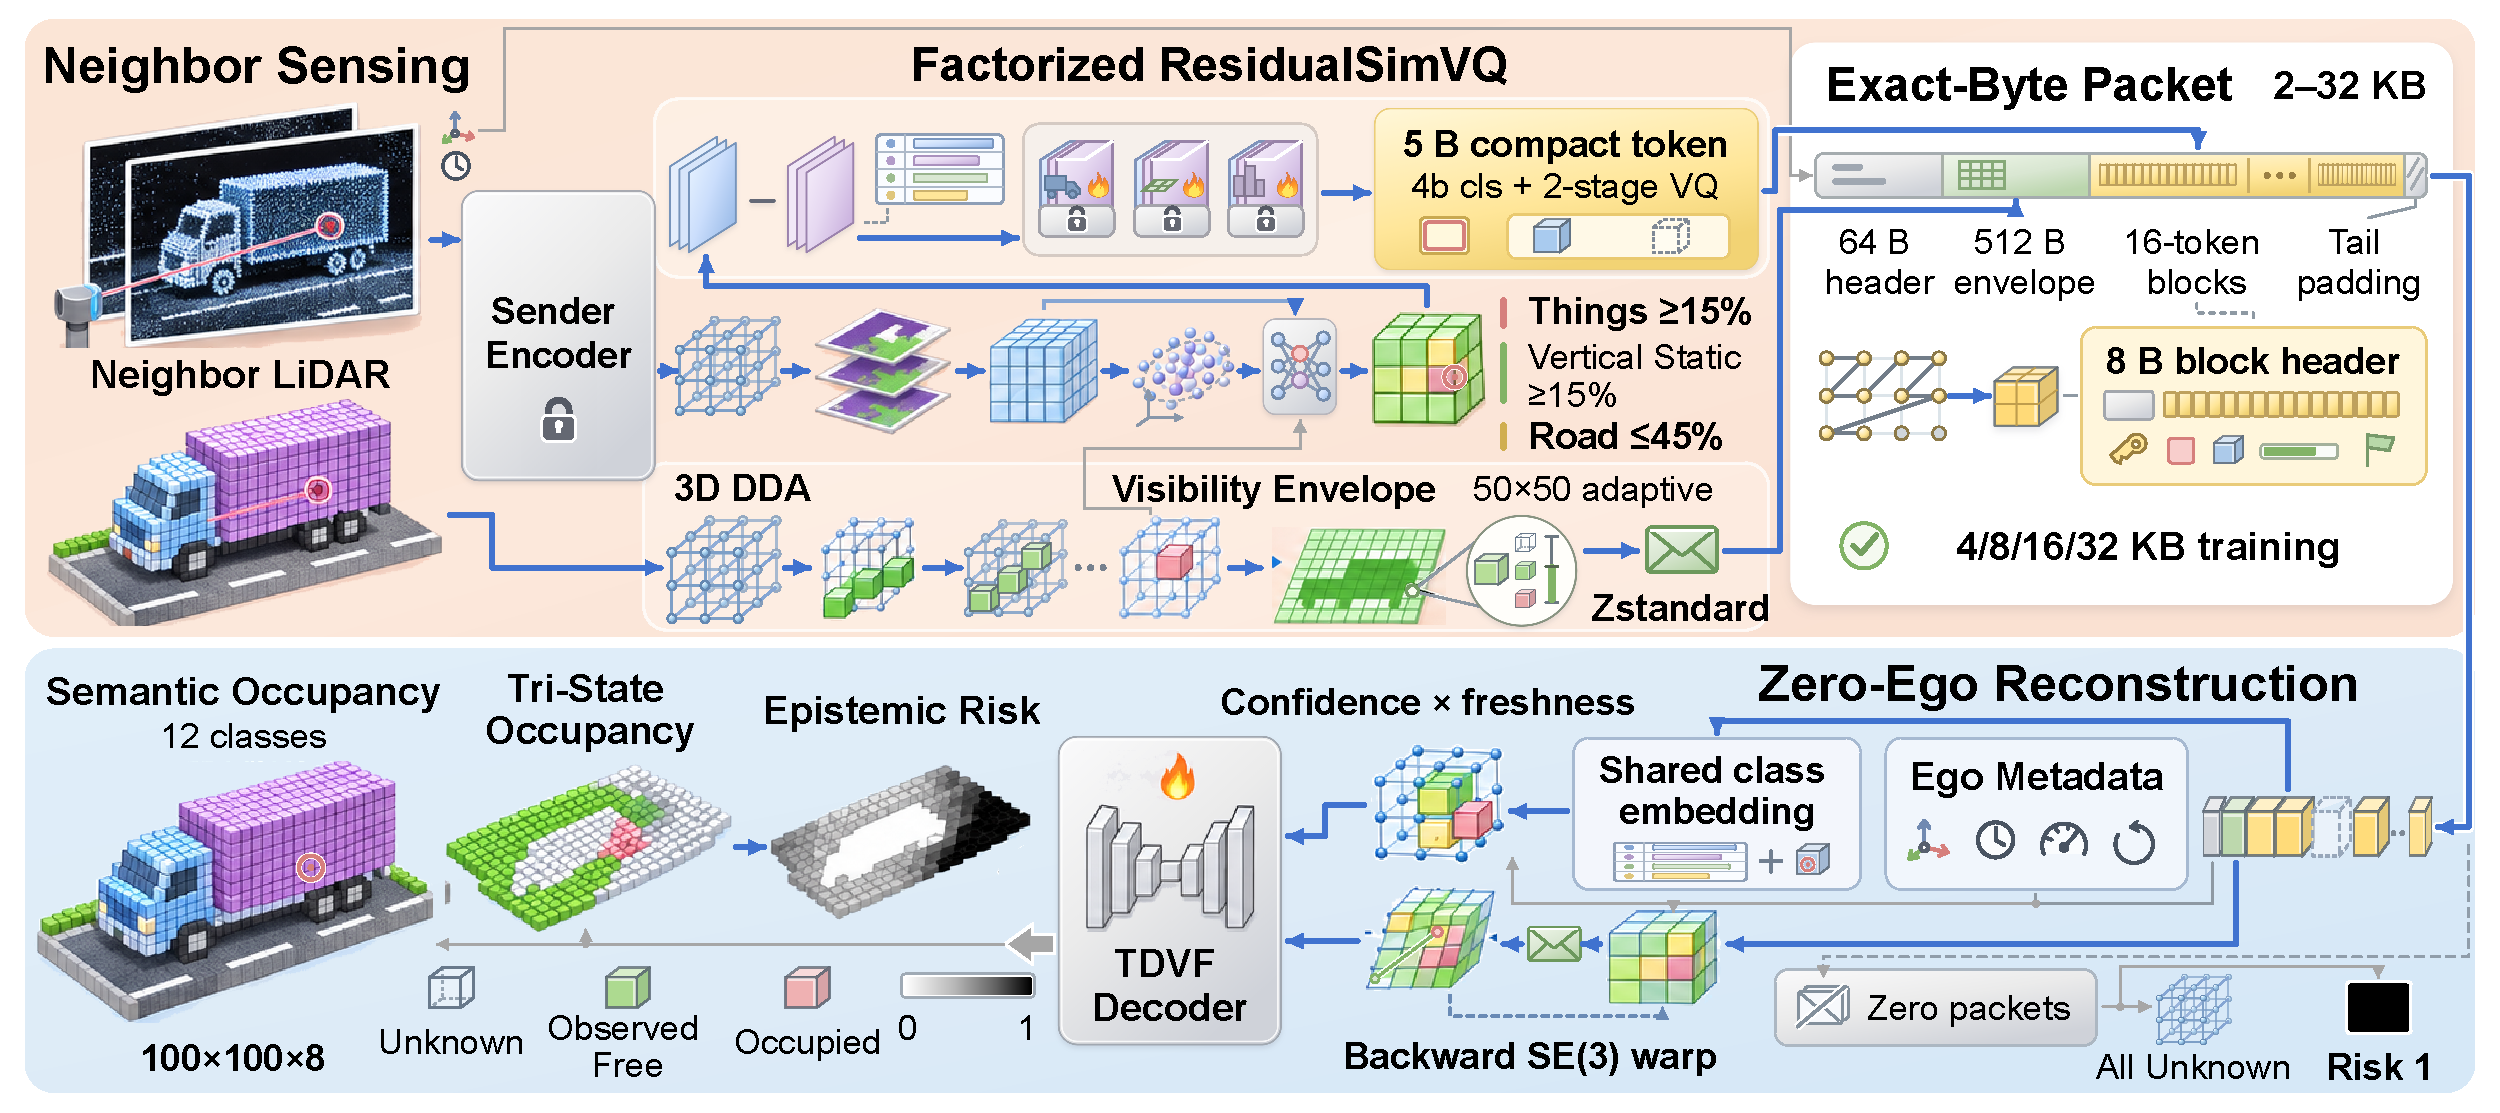
\includegraphics[width=\textwidth]{figures_pub/fig1_architecture.pdf}
\caption{End-to-end BorrowedSight architecture and exact-byte V2X protocol. \textbf{Top (Neighbor Sensing and Packetization):} Each LiDAR-equipped neighbor runs a frozen pure-PyTorch \texttt{SenderEncoder}, enforces category-balanced quotas (Things $\ge 15\%$, Vertical Static $\ge 15\%$, Road $\le 45\%$), and applies Factorized ResidualSimVQ to pack each anchor into a zero-waste 5-byte (40-bit) record uniting a lossless 17-bit coordinate, 4-bit class ID, two 6-bit geometry-group codes, and 7-bit confidence. Simultaneously, 3D DDA ray tracing constructs an adaptive $50\times 50$ visibility envelope plus $25\times 25$ max-height prior compressed via Zstd into a fixed 512~B slot alongside a 64~B packet header, self-contained 16-token Morton micro-blocks (8~B block header each), and exact tail padding across 2--32~KB links trained over randomized 4/8/16/32~KB budgets. \textbf{Bottom (Zero-Ego Reconstruction):} Flowing right-to-left, the receiver ingests strictly surviving micro-blocks and ego metadata, reconstructs additive factorized embeddings via the shared class embedding and confidence$\times$freshness fusion, backward-warps each Zstd visibility envelope via exact $\mathrm{SE}(3)$ geometry into a late-fusion TDVF tri-state refinement branch (or triggers a deterministic All-Unknown / Risk~1 fallback on zero packets), and decodes the $100\times 100\times 8$ volume into 12-class semantic occupancy, tri-state occupancy, and calibrated epistemic risk.}
\label{fig:architecture}
\end{figure*}

\subsection{Pure-PyTorch Sender Encoding and Category-Aware Quota Selection}

To enable portable deployment without fragile third-party sparse-convolution builds (such as \texttt{spconv} or \texttt{mmcv}), both sender and receiver run entirely in standard PyTorch. Each neighbor point cloud $\mathcal{P}_s$ inside the $100\times 100\times 8$ volume is aggregated per voxel $\mathbf{u} = (i_x, i_y, i_z)$ through differentiable scatter-mean pooling over local point offsets and normalized occupancy features~\cite{lang2019pointpillars}. The 3D volume is height-collapsed along $z$ into a BEV feature map, processed by a three-scale residual U-Net~\cite{ronneberger2015unet} with scaled dot-product self-attention at the $25\times 25$ bottleneck, and lifted back to $G_x \times G_y \times G_z$ to yield per-voxel embeddings $\mathbf{f}_u \in \mathbb{R}^{d}$ ($d = 16$) and local semantic predictions $\hat{c}_u \in \{1,\dots,12\}$.

For every ray-verified occupied voxel ($V_s(\mathbf{u}) = 2$), six geometric descriptors $\mathbf{g}_u \in \mathbb{R}^{6}$ (normalized point density, within-voxel centroid offset $(\delta x, \delta y, \delta z)$, and vertical/planar variance) are fused with appearance features via a two-layer multilayer perceptron (MLP) to produce a category-geometry latent $\mathbf{z}_u \in \mathbb{R}^d$ and importance score $s_u$:
\begin{equation}
\mathbf{z}_u = \phi_{\mathrm{fuse}}\!\left([\mathbf{f}_u \,\|\, \mathbf{g}_u]\right), \qquad s_u = \mathbf{w}_s^\top \mathbf{z}_u + b_s.
\label{eq:geo_fuse}
\end{equation}

In real multi-lane driving sweeps, planar road voxels constitute the majority of occupied LiDAR returns and quickly crowd out dynamic vehicles and thin vertical hazards under unconstrained top-$N$ selection. BorrowedSight therefore partitions the 12 semantic classes into three geometric super-groups: \textit{Things} ($\mathcal{G}_0$: Vehicles), \textit{Ground} ($\mathcal{G}_1$: Road, SideWalk, Terrain), and \textit{Vertical Static} ($\mathcal{G}_2$: Building, Fence, Pole, Vegetation, Wall, GuardRail, TrafficSign, Bridge). Given packet slot capacity $N(B)$, a zero-synchronization GPU-vectorized quota selector reserves minimum floors $\rho_{\mathrm{thing}} = 0.15$ for $\mathcal{G}_0$, $\rho_{\mathrm{vert}} = 0.15$ for $\mathcal{G}_2$, and a minimal road-continuity floor $\rho_{\mathrm{road,min}} = 0.10$ for low-bitrate links, prioritizes highest-scoring non-road anchors ahead of road anchors, and caps road tokens at $\rho_{\mathrm{road}} = 0.45$ via $N_{\mathrm{road}} \le \lfloor N_{\mathrm{other}} \rho_{\mathrm{road}} / (1 - \rho_{\mathrm{road}}) \rfloor$.

\subsection{Additive Category-Geometry Factorization and Zero-Waste 5-Byte Coding}

A subtle structural bottleneck arises when coupling discrete class tags with grouped vector quantizers. Even when three separate geometry codebooks $\mathcal{Q}_g$ ($g \in \{0,1,2\}$, $K_{\mathrm{cb}} = 32$ prototypes per stage) are assigned to Things, Ground, and Vertical Static, the Vertical Static group spans eight structurally distinct classes (from wide building facades to slender poles and traffic signs). If the receiver uses the transmitted class tag $c_u$ solely to select group $g(c_u)$ and discards $c_u$ during feature reconstruction, those eight classes compete for 32 shared geometry vectors, degrading vertical-class recognition.

BorrowedSight eliminates this bottleneck through \textbf{Additive Category-Geometry Factorization}. Both sender and receiver share a lightweight learnable category embedding table $\mathbf{E}_{\mathrm{cls}} \in \mathbb{R}^{13 \times d}$ (just 208 parameters and \textit{zero extra wire bits}). On the sender side, the fused latent $\mathbf{z}_u$ enters group $g = g(c_u)$ directly via a two-stage ResidualSimVQ codebook~\cite{zeghidour2021soundstream,zhu2025simvq} trained with the rotation trick~\cite{fifty2025rotation}, starting from $\mathbf{r}_u^{(0)} = \mathbf{z}_u$:
\begin{equation}
q_u^{(\ell)} = \arg\min_{k \in \{1,\dots,K_{\mathrm{cb}}\}} \left\|\mathbf{r}_u^{(\ell-1)} - \mathbf{W}_g^{(\ell)} \mathbf{e}_{g,k}^{(\ell)}\right\|_2^2,
\label{eq:rvq_index}
\end{equation}
\begin{equation}
\begin{aligned}
\mathbf{r}_u^{(\ell)} &= \mathbf{r}_u^{(\ell-1)} - \mathbf{W}_g^{(\ell)} \mathbf{e}_{g,q_u^{(\ell)}}^{(\ell)}, \\
\hat{\mathbf{z}}_u^{(S)} &= \mathbf{E}_{\mathrm{cls}}(c_u) + \sum_{\ell=1}^{S} \mathbf{W}_g^{(\ell)} \mathbf{e}_{g,q_u^{(\ell)}}^{(\ell)},
\end{aligned}
\label{eq:rvq_recon}
\end{equation}
where $\mathbf{e}_{g,k}^{(\ell)} \in \mathbb{R}^d$ are frozen bases and $\mathbf{W}_g^{(\ell)} \in \mathbb{R}^{d\times d}$ is the learnable SimVQ projection matrix. Avoiding un-detached subtraction of $\mathbf{E}_{\mathrm{cls}}(c_u)$ prior to Eq.~\eqref{eq:rvq_index} is critical in practice: subtracting $\mathbf{E}_{\mathrm{cls}}(c_u)$ inside the VQ commitment objective lets gradients drive $\mathbf{z}_u - \mathbf{E}_{\mathrm{cls}}(c_u) \to \mathbf{0}$ and collapses over 70\% of codebook prototypes, whereas additive reconstruction in Eq.~\eqref{eq:rvq_recon} maintains healthy 0.73--0.80 codebook utilization while explicitly anchoring exact class identity on sender and receiver.

Standard byte-aligned token formats waste over one-third of every record on oversized 32-bit coordinates, 8-bit class fields for 13 categories, and unused byte padding (8--9~B/token). BorrowedSight eliminates this waste through \textbf{zero-waste 5-byte (40-bit) compact bit-packing}. On the $100\times 100\times 8$ volume, exact voxel coordinates require only $7 + 7 + 3 = 17$ bits via lossless coordinate packing $p(i_x, i_y, i_z) = i_x \mid (i_y \ll 7) \mid (i_z \ll 14)$. Packing all fields tightly into one 40-bit record allocates exact bit widths with \textit{zero wasted bits}:
\begin{equation}
\underbrace{17\text{ b}}_{\text{coord } p(\mathbf{u})} + \underbrace{4\text{ b}}_{\text{cls } c_u} + \underbrace{6\text{ b}}_{\text{code } q_u^{(1)}} + \underbrace{6\text{ b}}_{\text{code } q_u^{(2)}} + \underbrace{7\text{ b}}_{\text{conf } \hat{\pi}_u} = 40\text{ bits } (5\text{ B}).
\label{eq:bitpack}
\end{equation}
For compression efficiency, this 40-bit layout carries \textit{both} Stage-1 and Stage-2 residual VQ codes ($S=2$) inside 5~bytes, making Stage-2 geometric refinement completely free in packet bytes while raising spatial token density by $+54\%$ relative to 8-byte tokens (5,840 tokens at 32~KB and 2,864 at 16~KB for \textbf{B4-TDVF}, or 5,936 tokens at 32~KB for envelope-free \textbf{B4-Compact}). To preserve strict equal-byte fairness, our shared-VQ baseline (\textbf{B3}) receives the analogous compact \textbf{4-byte (32-bit)} layout ($17\text{ b coord} + 6\text{ b code} + 8\text{ b conf} + 1\text{ b pad}$), granting B3 7,264 tokens at 32~KB (+24.4\% more spatial anchors than B4-TDVF) and 3,616 tokens at 16~KB.

\subsection{Morton Micro-Blocks and Adaptive $50\times 50$ Zstd Visibility Envelopes}

To withstand bursty V2X packet drops without cross-packet desynchronization, selected anchors are spatially ordered by their exact 20-bit 3D Morton Z-order key~\cite{morton1966zorder} computed in $\mathcal{O}(1)$ via precomputed lookup tables:
\begin{equation}
m(i_x, i_y, i_z) = \sum_{b=0}^{6} \left(2^{3b} i_{x,b} + 2^{3b+1} i_{y,b}\right) + \sum_{b=0}^{2} 2^{3b+2} i_{z,b}.
\label{eq:morton}
\end{equation}
Every 16 consecutive anchors form a self-contained micro-block carrying an 8-byte block header (starting Morton key, valid token count, padding flag) and 16 compact records (88~B/block for 5-byte B4, 72~B/block for 4-byte B3). Dropping any subset of micro-blocks leaves all surviving blocks independently decodable because each record carries its lossless 17-bit absolute voxel coordinate $p(\mathbf{u})$.

To transmit verified free-space and occlusion boundaries at zero wire-budget penalty, \textbf{B4-TDVF} reserves a fixed 512-byte visibility slot (3 framing bytes plus up to 509 Zstd payload bytes). Earlier coarse $20\times 20$ ($2.0\,\mathrm{m}$) and $25\times 25$ ($1.6\,\mathrm{m}$) envelopes consumed only 104--190~B after Zstandard compression, leaving over 320~B idle inside the fixed slot. BorrowedSight exploits this unused slot headroom via an \textbf{adaptive multi-resolution visibility payload}:
\begin{enumerate}
\item \textit{Primary ($50\times 50$ bit-planes + $25\times 25$ $z_{\max}$, 1,252~B raw):} Three bit-packed $50\times 50$ ($0.8\,\mathrm{m}$, $4\times$ denser than $25\times 25$) boolean planes indicating column-wise Observed Free, Occupied, and Unknown presence (939~B) concatenated with nibble-packed $25\times 25$ maximum occupied height bins $z_{\max} \in \{0,\dots,7\}$ (313~B).
\item \textit{Graceful fallback ($50\times 50$ bit-planes only, 939~B raw, or $25\times 25$, 625~B raw):} Whenever a highly cluttered sweep exceeds 509~B at Zstd level~3/9 in Tier~1, the packer deterministically drops the $z_{\max}$ nibbles and compresses the 939~B $50\times 50$ bit-planes (falling back to $25\times 25$ only if 939~B still exceeds 509~B).
\end{enumerate}
Across all \textbf{4,736} real OPV2V clear sender sweeps (train, validate, and test), \textbf{100.0\%} fit inside the fixed 512~B slot at full $50\times 50$ resolution (compressed size 295--509~B, mean \textbf{433.5~B}): 3,285 sweeps (69.4\%) carry both $50\times 50$ bit-planes and $25\times 25$ $z_{\max}$ height priors, 1,451 sweeps (30.6\%) fall back cleanly to $50\times 50$ bit-planes, and 0 sweeps (0.0\%) ever degrade to $25\times 25$. Sub-block tail padding locks $\epsilon_{\mathrm{byte}} = 0.0\%$ across all methods (exact binary layout in \ref{app:wire}, Table~\ref{tab:app_wire}).

\subsection{Task-Decoupled Visibility Fusion (TDVF) and Safety-Aware Training}

Upon receiving packets $\{b_s\}_{s \in \mathcal{S}}$ at time $t$, the zero-ego receiver unpacks surviving micro-blocks via vectorized bit extraction, reconstructs factorized embeddings $\hat{\mathbf{z}}_u^{(S)}$ via Eq.~\eqref{eq:rvq_recon}, transforms anchor coordinates into ego coordinates via Eq.~\eqref{eq:se3_transform}, and weights multi-sender evidence by quantized confidence and temporal freshness decay:
\begin{equation}
w_{s,u} = \hat{\pi}_{s,u} \cdot \exp\!\left(-\frac{|t - t_s|}{\tau}\right), \qquad \tau = 0.5\,\mathrm{s}.
\label{eq:age_weight}
\end{equation}
Each sender's adaptive $50\times 50$ visibility envelope and $25\times 25$ $z_{\max}$ prior are mapped into the $100\times 100$ ego BEV grid via exact backward $\mathrm{SE}(3)$ warping rather than direct array blitting. Every ego BEV cell center $\mathbf{x}_E = (x_E, y_E, 0)^\top$ maps back into sender $s$'s local frame:
\begin{equation}
\tilde{\mathbf{x}}_{E \to s} = \left(\mathbf{T}_s^W\right)^{-1} \mathbf{T}_E^W \tilde{\mathbf{x}}_E,
\label{eq:env_warp}
\end{equation}
followed by bounds-checked lookup to produce a 4-channel visibility/height tensor $\mathbf{C}_{\mathrm{vis}} \in \mathbb{R}^{4 \times 100 \times 100}$ (Observed Free, Occupied, Unknown, and normalized $z_{\max}/7$) alongside a 4-channel token/motion tensor $\mathbf{C}_{\mathrm{tok}} \in \mathbb{R}^{4 \times 100 \times 100}$ (auxiliary sensor-origin ray carving from $\mathbf{o}_{s \to E}$, mean packet age, and ego kinematics $\mathbf{m}_E$).

\textbf{Task-Decoupled Visibility Fusion (TDVF).} Upgrading the receiver U-Net with Group Normalization~\cite{wu2018groupnorm} and fixed 2D sinusoidal positional encodings at the $25\times 25$ self-attention bottleneck stabilizes cross-scene decoding across all methods (B1--B4). A critical phenomenon emerges when feeding dense $50\times 50$ visibility and $z_{\max}$ channels directly into the shared semantic U-Net stem: because $\mathbf{C}_{\mathrm{vis}}$ correlates tightly with scene geometry on training corridors, the semantic branch exploits it as a geometric shortcut, driving training cross-entropy $4\times$ lower yet hurting held-out test mIoU by $-1.39$ points (Table~\ref{tab:ablation}) and elevating blind-zone errors. \textbf{TDVF} resolves this conflict structurally by routing only sparse token volume $\mathbf{F}_E$ and $\mathbf{C}_{\mathrm{tok}}$ into the shared U-Net decoder to produce semantic logits $\hat{\mathbf{Y}}_{\mathrm{sem}}$ and coarse tri-state features $\mathbf{H}_{\mathrm{dec}}$, while a lightweight 74.7K-parameter late-fusion residual block $\psi_{\mathrm{vis}}$ fuses $\mathbf{C}_{\mathrm{vis}}$ exclusively into the tri-state occupancy head:
\begin{equation}
\hat{\mathbf{Y}}_{\mathrm{tri}} = \phi_{\mathrm{tri}}\!\left(\mathbf{H}_{\mathrm{dec}} + \psi_{\mathrm{vis}}\!\left([\mathbf{H}_{\mathrm{dec}} \,\|\, \mathbf{C}_{\mathrm{vis}}]\right)\right).
\label{eq:tdvf}
\end{equation}
This strict pathway separation guarantees mathematically that semantic logits remain immune to envelope-induced shortcut overfitting while tri-state boundaries exploit the full $50\times 50$ visibility and $z_{\max}$ prior. During training, dropping $z_{\max}$ on 16\% of samples and masking $\mathbf{C}_{\mathrm{vis}}$ on 8\% aligns the late-fusion branch with Tier-2 Zstd fallback and partial link loss. Per-voxel epistemic risk merges normalized Shannon predictive entropy~\cite{shannon1948entropy,guo2017calibration} over the tri-state posterior $\mathbf{p}(\mathbf{u}) = \mathrm{softmax}(\hat{\mathbf{Y}}_{\mathrm{tri}}(\mathbf{u}))$ with unobserved posterior probability $p_0(\mathbf{u})$:
\begin{equation}
U(\mathbf{u}) = -\frac{1}{2\ln 3} \sum_{k=0}^{2} p_k(\mathbf{u}) \ln\!\left(p_k(\mathbf{u}) + \varepsilon\right) + \frac{1}{2} p_0(\mathbf{u}) \in [0, 1].
\label{eq:uncertainty}
\end{equation}

\textbf{IoU-Direct, Safety-Aware, and Multi-Budget Training.} To align optimization directly with both volumetric mIoU and blind-zone safety, all trainable receiver, fusion, scorer, category-embedding, and VQ parameters are optimized end-to-end with frozen sender weights via
\begin{equation}
\mathcal{L} = \mathcal{L}_{\mathrm{sem}}^{\mathrm{CE}} + \lambda_{\mathrm{lov}} \mathcal{L}_{\mathrm{sem}}^{\mathrm{Lov}} + \lambda_{\mathrm{tri}} \mathcal{L}_{\mathrm{tri}} + \lambda_{\mathrm{ufe}} \mathcal{L}_{\mathrm{ufe}} + \mathcal{L}_{\mathrm{vq}} + \lambda_{\mathrm{sc}} \mathcal{L}_{\mathrm{score}},
\label{eq:total_loss}
\end{equation}
where $\mathcal{L}_{\mathrm{sem}}^{\mathrm{Lov}}$ is masked multi-class Lov\'asz-Softmax~\cite{berman2018lovasz} ($\lambda_{\mathrm{lov}} = 0.5$), $\mathcal{L}_{\mathrm{ufe}} = -\mathbb{E}_{Y_{\mathrm{tri}}=0}[\ln(1 - p_1(\mathbf{u}) + \varepsilon)]$ is an asymmetric safety penalty that directly punishes predicting \textit{Observed Free} inside unobserved blind zones ($\lambda_{\mathrm{ufe}} = 0.35$), $\lambda_{\mathrm{tri}} = 0.5$, and $\lambda_{\mathrm{sc}} = 0.05$. Every training batch applies exact 8-way $D_4$ dihedral BEV augmentation (rotations and flips synchronized across $\mathbf{F}_E$, $\mathbf{C}_{\mathrm{tok}}$, $\mathbf{C}_{\mathrm{vis}}$, and 3D targets) together with mild V2X impairment exposure (12\% 1--5 frame latency, 15\% 10--35\% token drop, and 6\% $0.25\,\mathrm{m}/1^\circ$ pose jitter). For rate-adaptive deployment with a single checkpoint (\textbf{B4-TDVF-MultiBW}), each training sample draws its packet budget uniformly from $\{4096, 8192, 16384, 32768\}$ bytes. Algorithm~\ref{alg:borrowedsight} summarizes the complete pipeline.

\begin{algorithm}[t]
\caption{BorrowedSight Zero-Ego V2X Occupancy Pipeline}
\label{alg:borrowedsight}
\KwIn{Neighbor sweeps $\{\mathcal{P}_s, \mathbf{T}_s^W, t_s\}_{s \in \mathcal{S}}$ ($E \notin \mathcal{S}$); ego metadata $(\mathbf{T}_E^W, t, \mathbf{m}_E)$; byte budget $B$; compact flag.}
\KwOut{Ego 3D semantic occupancy $\hat{\mathbf{Y}}_{\mathrm{sem}}$, tri-state $\hat{\mathbf{Y}}_{\mathrm{tri}}$, risk $U$.}
\BlankLine
\tcp{Phase 1: Neighbor Sender Encoding \& Compact Packing}
Initialize packet set $\mathcal{B} \leftarrow \emptyset$\;
\ForEach{neighbor sender $s \in \mathcal{S}$}{
  Compute voxel features $\mathbf{f}$ and local classes $\hat{c}$ via frozen \texttt{SenderEncoder}($\mathcal{P}_s$)\;
  Trace sender rays from $\mathbf{0}$ to $\mathcal{P}_s$ to build tri-state grid $V_s$, $50\times 50$ bit-planes, and $25\times 25$ $z_{\max}$\;
  Fuse 6-d local geometry $\mathbf{g}_u$ with $\mathbf{f}_u$ via Eq.~\eqref{eq:geo_fuse} to obtain $\mathbf{z}_u$ and logits $s_u$\;
  Select $N(B)$ occupied anchors via vectorized category quotas ($\rho_{\mathrm{thing}}, \rho_{\mathrm{vert}}, \rho_{\mathrm{road}}$)\;
  Quantize $\mathbf{z}_u$ via 2-stage group codebook $\mathcal{Q}_{g(\hat{c}_u)}$ using Eqs.~\eqref{eq:rvq_index}--\eqref{eq:rvq_recon}\;
  Sort anchors by 20-bit Morton key Eq.~\eqref{eq:morton}, bit-pack 40-bit records Eq.~\eqref{eq:bitpack} into 16-token micro-blocks with adaptive 512~B Zstd envelope and exact tail padding to size $B$, and transmit $b_s$\;
  Append surviving received packet $b_s$ (after channel drops) to $\mathcal{B}$\;
}
\BlankLine
\tcp{Phase 2: Strict Zero-Ego TDVF Receiver Reconstruction}
\If{$\mathcal{B} = \emptyset$}{
  \Return{safe fallback: 100\% \textit{Unknown} ($\mathrm{UFE}=0.0$) and maximal risk}\;
}
Initialize ego volume $\mathbf{F}_E \leftarrow \mathbf{0}$, weight $\mathbf{W}_E \leftarrow \mathbf{0}$, contexts $\mathbf{C}_{\mathrm{tok}}, \mathbf{C}_{\mathrm{vis}} \leftarrow \mathbf{0}$\;
\ForEach{received packet $b_s \in \mathcal{B}$}{
  Unpack surviving micro-blocks and reconstruct additive $\hat{\mathbf{z}}_u^{(2)} = \mathbf{E}_{\mathrm{cls}}(c_u) + \mathrm{VQ}_{g}(q_u^{(1)}, q_u^{(2)})$\;
  Warp anchor coordinates via Eq.~\eqref{eq:se3_transform} and scatter-accumulate weighted features Eq.~\eqref{eq:age_weight}\;
  Backward-warp adaptive $50\times 50$ envelope and $z_{\max}$ into $\mathbf{C}_{\mathrm{vis}}$ via Eq.~\eqref{eq:env_warp} and carve auxiliary rays into $\mathbf{C}_{\mathrm{tok}}$\;
}
Normalize $\mathbf{F}_E \leftarrow \mathbf{F}_E / \max(\mathbf{W}_E, 10^{-6})$, decode semantic logits $\hat{\mathbf{Y}}_{\mathrm{sem}}$ from $(\mathbf{F}_E, \mathbf{C}_{\mathrm{tok}})$, and refine tri-state $\hat{\mathbf{Y}}_{\mathrm{tri}}$ via TDVF Eq.~\eqref{eq:tdvf}\;
Compute epistemic risk $U$ via Eq.~\eqref{eq:uncertainty}\;
\Return{$(\hat{\mathbf{Y}}_{\mathrm{sem}}, \hat{\mathbf{Y}}_{\mathrm{tri}}, U)$}\;
\end{algorithm}

\section{Experiments and Analysis}

With the zero-ego communication protocol and vectorized architecture established in Section~4, we validate BorrowedSight across five complementary tiers: (1) a 9-scene real OPV2V multi-sender physical visibility oracle, (2) full 25-scene multi-sender real OPV2V and Mini-200 equal-byte comparisons, (3) strict scene-grouped 5-fold cross-validation across all 25 disjoint scenes, (4) orthogonal component ablations, codebook sensitivity, and multi-seed stability, and (5) bandwidth scaling (2--32~KB), LISA physical weather, multi-sender scaling, urban congestion, V2X impairments, qualitative analysis, and real-time RTX~3090 profiling.

\subsection{Datasets, Baselines, and Reproducible Compute Setup}

\textbf{Full Multi-Sender Real OPV2V + Semantic-OPV2V Benchmark.} We pair raw OPV2V~\cite{xu2022opv2v} multi-CAV LiDAR point clouds and degree-accurate 6-DoF poses with official Semantic-OPV2V (\texttt{4LidarSurround}) voxel labels~\cite{song2024cohff} over the exact $100\times 100\times 8$ CoHFF volume. Following strict scene-level separation (zero scene or temporal overlap across splits), our real benchmark comprises \textbf{25 complete driving scenarios (2,383 multi-CAV frames, 2--5 CAVs per scene)}:
\begin{itemize}
\item \textbf{Train (13 scenes, 1,084 frames):} 2--4 CAVs per scene (mean 2.62 CAVs, 0--11 vehicles/frame), covering all \textbf{12/12} semantic foreground classes.
\item \textbf{Validate (6 scenes, 573 frames):} 2--5 CAVs per scene (mean 2.67 CAVs, 1--10 vehicles/frame), covering all \textbf{12/12} semantic foreground classes.
\item \textbf{Held-Out Test (6 scenes, 726 frames):} 2--5 CAVs per scene (mean 3.33 CAVs, 5 of 6 scenes multi-sender with 3--5 CAVs, 1--11 vehicles/frame), covering \textbf{11/12} foreground classes plus Observed Free (only \textit{Bridge} is physically absent from these 6 test scenes).
\end{itemize}
Coordinate audit confirms 25/25 (100.0\%) ground-truth vehicle centers falling on semantic \textit{Vehicles} voxels and 98.82\% of raw neighbor LiDAR points landing on occupied semantic voxels. For full 25-scene statistical validation, we additionally partition all 25 scenarios into 5 load-balanced, strictly disjoint 5-scene folds (470--483 validation frames per fold). As a controlled secondary protocol benchmark, we also evaluate on the 200-frame, 3-sender \textbf{Mini-200} suite. Training uses exclusively clear sweeps with lightweight 1~cm jitter and 5\% random drop~\cite{park2024lidarweather}. Physics-based \textbf{LISA}~\cite{kilic2021lisa} Beer--Lambert fog and Monte Carlo rain are strictly held out in physically separate test caches (total sparse cache footprint 1.61~GB).

\textbf{Frozen Sender Backbone and Equal-Capacity Baselines.} The shared pure-PyTorch \texttt{SenderEncoder} (1.170M parameters, 7.64 giga floating-point operations, GFLOPs) is trained for 30 epochs on the 13 real training scenes (2,571.3~s / 0.71~GPU-h, 0.25~GB peak VRAM), achieving \textbf{0.7150} validation mIoU across all 13/13 classes (Vehicle IoU \textbf{0.9133}, Road IoU \textbf{0.9757}, Building IoU \textbf{0.9107}, GuardRail IoU \textbf{0.9501}). All transmitting methods share this exact frozen encoder, the exact GroupNorm + 2D-PE \texttt{ReceiverDecoder} backbone, the identical Lov\'asz + UFE + $D_4$ + mild-impairment training recipe, and the exact micro-block packer:
\begin{itemize}
\item \textbf{B0 (No Communication):} 0~B received, establishing the strict zero-ego lower bound.
\item \textbf{B1 (Sparse FP16):} Top-$k$ geometry-salient anchors transmit raw 16-d 16-bit floating-point (FP16) vectors at 36~B/token (432 tokens at 16~KB, 896 at 32~KB).
\item \textbf{B2 (Projected Continuous):} Learned top-$k$ anchors project to 8-d FP16 vectors at 20~B/token (784 tokens at 16~KB, 1,584 at 32~KB).
\item \textbf{B3 (Compact 4B Shared VQ):} Learned top-$k$ anchors use a single shared ResidualSimVQ codebook, adapting the sparse-aware quantization of VQSOP~\cite{li2026vqsop} to identical LiDAR backbones with compact 4~B/token bit-packing (3,616 tokens at 16~KB, 7,264 at 32~KB).
\item \textbf{B4-Compact and B4-TDVF (BorrowedSight):} Full zero-waste 5~B/token Stage-2 category-geometry factorized protocol with 3-group ResidualSimVQ, 208-parameter class embeddings, and category quotas. \textbf{B4-Compact} omits the 512~B envelope slot to maximize clear-weather token count (5,936 tokens at 32~KB, identical 15.22~GFLOPs decoder), whereas \textbf{B4-TDVF} reserves the fixed 512~B adaptive $50\times 50$ Zstd visibility slot (2,864 tokens at 16~KB, 5,840 at 32~KB) paired with late-fusion TDVF tri-state refinement (\textbf{B4-TDVF-MultiBW} adds 4--32~KB randomized budget training).
\end{itemize}

\textbf{Metrics and RTX~3090 Compute Budget.} Semantic reconstruction is scored by mIoU over Observed Free and all present CoHFF classes within neighbor-observed ground truth, alongside \textit{Vehicle IoU} and \textit{Road IoU}. Safety-boundary integrity is measured by \textit{Unknown F1} and \textit{UFE}---the fraction of ground-truth unobserved blind voxels mispredicted as free space. Table~\ref{tab:config} summarizes exact parameter counts, FLOPs, hyperparameters, and single-GPU RTX~3090 training budgets. \textbf{B4-Compact} adds only \textbf{1,232 parameters (+0.053\%)} over compact B3 (+1,024 for grouped codebooks and +208 for $\mathbf{E}_{\mathrm{cls}}$) at identical 15.22~GFLOPs, while \textbf{B4-TDVF} adds 74.7K parameters (+3.24\% total, 16.70~GFLOPs) for the late-fusion visibility branch. Receivers train for 20 epochs (batch size 4, bfloat16 decoder autocast, AdamW~\cite{loshchilov2019adamw} at $\mathrm{lr} = 8\times 10^{-4}$, cosine decay, gradient clip 5.0) in 6.0--20.2~min per model on an idle RTX~3090 at peak VRAM $\le 0.52$~GB.

\begin{table*}[!tbp]
\centering
\caption{Exact model capacity, computational footprint, training cost, and shared hyperparameters measured on a single NVIDIA RTX~3090 GPU (PyTorch 2.10.0+cu128). \textbf{B4-Compact} adds only 1,232 parameters (+0.053\%) over compact B3 at identical 15.22~GFLOPs, while \textbf{B4-TDVF} adds 74.7K late-fusion visibility parameters (+3.24\%).}
\label{tab:config}
\resizebox{\textwidth}{!}{%
\begin{tabular}{lrrrrcll}
\toprule
\textbf{Method} & \textbf{Encoder} & \textbf{Decoder} & \textbf{Comm. Head} & \textbf{Total Params} & \textbf{Token Width} & \textbf{Compute \& Training Budget (RTX 3090)} & \textbf{Shared Hyperparameters} \\
\midrule
B0 (No Comm) & 1,170,040 & 1,169,280 & 657 & 2,339,977 & 0~B & Sender GFLOPs: \textbf{7.64} \quad Base Dec. GFLOPs: \textbf{7.58} & Grid: $100\times 100\times 8$ ($40\times 40\times 3.4$~m) \\
B1 (Sparse FP16) & 1,170,040 & 1,169,280 & 657 & 2,339,977 & 36~B & Total GFLOPs: \textbf{15.22} (B0--B4-Compact) / \textbf{16.70} (TDVF) & Feature dim $d = 16$, codebook $K_{\mathrm{cb}} = 32$ \\
B2 (Cont. 8-d) & 1,170,040 & 1,169,280 & 937 & 2,340,257 & 20~B & Real sender (30 ep, 13 scenes): \textbf{0.71~GPU-h} (249~MB) & Optimizer: AdamW ($\mathrm{wd} = 10^{-4}$, clip $5.0$) \\
B3 (Compact 4B VQ) & 1,170,040 & 1,169,280 & 1,169 & 2,340,489 & 4~B & Idle 20-ep receiver (bs=4): \textbf{6.0--20.2~min} ($\le 0.52$~GB) & Real LR: $6\times 10^{-4}$ (tx) / $8\times 10^{-4}$ (rx) \\
\rowcolor{oursrow}
\textbf{B4-Compact (Ours)} & \textbf{1,170,040} & \textbf{1,169,280} & \textbf{2,401} & \textbf{2,341,721} & \textbf{5~B (S2)} & Losses: $\lambda_{\mathrm{lov}}=0.5$, $\lambda_{\mathrm{tri}}=0.5$, $\lambda_{\mathrm{ufe}}=0.35$ & Quotas: $\rho_{\mathrm{road}}=0.45$, $\rho_{\mathrm{thing}}=\rho_{\mathrm{vert}}=0.15$ \\
\rowcolor{oursrow}
\textbf{B4-TDVF (Ours)} & \textbf{1,170,040} & \textbf{1,243,968} & \textbf{2,401} & \textbf{2,416,409} & \textbf{5~B (S2)} & 5-Fold CV (20 models, 25 scenes): \textbf{6.69~GPU-h} & Aug.: $8\times D_4$ BEV + mild V2X impairments \\
\bottomrule
\end{tabular}}
\end{table*}

\subsection{Multi-Sender Visibility Oracle on Real OPV2V}

Before evaluating neural communication, we quantify the physical observation ceiling across all 9 real OPV2V validation scenes (90 frames, exact degree-based $\mathrm{SE}(3)$ ray tracing). Table~\ref{tab:oracle} and Fig.~\ref{fig:oracle} first establish the strong multi-sender dividend on dynamic traffic targets: expanding the cooperating fleet from 1 to 3 clear-weather senders lifts 3D vehicle box recall from 0.7962 to \textbf{0.9190} while pushing near-range coverage (0--10~m) from 0.4617 to \textbf{0.4962}. Stratifying clear frames by urban traffic density reveals a counterintuitive cooperative advantage: rather than degrading visibility, dense vehicle fleets convert inter-vehicle occlusion into complementary multi-view observation angles, driving medium-density recall to 0.9684 and dense-traffic recall to \textbf{1.0000} alongside an observable coverage jump from 0.5036 to 0.5850.

Weather attenuation and persistent blind volume simultaneously expose why standard occupied-versus-empty formulations fail physically in zero-ego driving. Under LISA rain and fog, aerosol extinction and droplet backscatter sharply shorten neighbor laser penetration, inflating unobservable blind volume from 61.22\% (clear, 1 sender) to 72.30\%--76.35\% in rain and \textbf{88.42\%--90.18\%} in fog while lowering fog vehicle recall to 0.5043--0.5837. Even under ideal clear weather with three active LiDAR senders, \textbf{58.70\%} of the ego grid remains physically unsampled by any ray, proving that explicit \textit{Unknown} visibility modeling is a physical requirement rather than an optional refinement.

\begin{table*}[!tbp]
\centering
\caption{Physical multi-sender visibility oracle across all 9 real OPV2V validation scenes (90 frames). Even with three clear-weather senders, 58.70\% of ego voxels remain physically unobservable, and LISA fog drives blind volume above 88\%.}
\label{tab:oracle}
\resizebox{\textwidth}{!}{%
\begin{tabular}{llccccc}
\toprule
\textbf{Stratification} & \textbf{Regime} & \textbf{Active Senders} & \textbf{Observable Coverage} & \textbf{Unknown Volume} & \textbf{3D Vehicle Box Recall} & \textbf{Near-Range Coverage (0--10~m)} \\
\midrule
Weather & Clear & 1 / 2 / 3 & 0.3878 / 0.3799 / \textbf{0.4130} & 0.6122 / 0.6201 / \textbf{0.5870} & 0.7962 / \underline{0.8836} / \textbf{0.9190} & 0.4617 / \underline{0.4768} / \textbf{0.4962} \\
Weather & LISA Rain & 1 / 2 / 3 & 0.2365 / \underline{0.2523} / \textbf{0.2770} & 0.7635 / \underline{0.7477} / \textbf{0.7230} & \textbf{0.8560} / \underline{0.7982} / 0.7844 & 0.3003 / \underline{0.3088} / \textbf{0.3173} \\
Weather & LISA Fog & 1 / 2 / 3 & 0.0982 / \underline{0.1028} / \textbf{0.1158} & 0.9018 / \underline{0.8972} / \textbf{0.8842} & 0.5043 / \underline{0.5574} / \textbf{0.5837} & 0.1172 / \underline{0.1174} / \textbf{0.1239} \\
\midrule
Traffic Density (Clear) & Sparse & 1 / 2 / 3 & \textbf{0.3813} / \underline{0.3224} / 0.2815 & \textbf{0.6187} / \underline{0.6776} / 0.7185 & \underline{0.7745} / \textbf{0.8013} / 0.7619 & -- \\
Traffic Density (Clear) & Medium & 1 / 2 / 3 & 0.3857 / \underline{0.4022} / \textbf{0.4572} & 0.6143 / \underline{0.5978} / \textbf{0.5428} & 0.8030 / \underline{0.9201} / \textbf{0.9684} & -- \\
\rowcolor{oursrow}
\textbf{Traffic Density (Clear)} & \textbf{Dense} & \textbf{1 / 2 / 3} & 0.5036 / \underline{0.5542} / \textbf{0.5850} & 0.4964 / \underline{0.4458} / \textbf{0.4150} & 0.9259 / \textbf{1.0000} / \textbf{1.0000} & -- \\
\bottomrule
\end{tabular}}
\end{table*}

\begin{figure*}[!tbp]
\centering
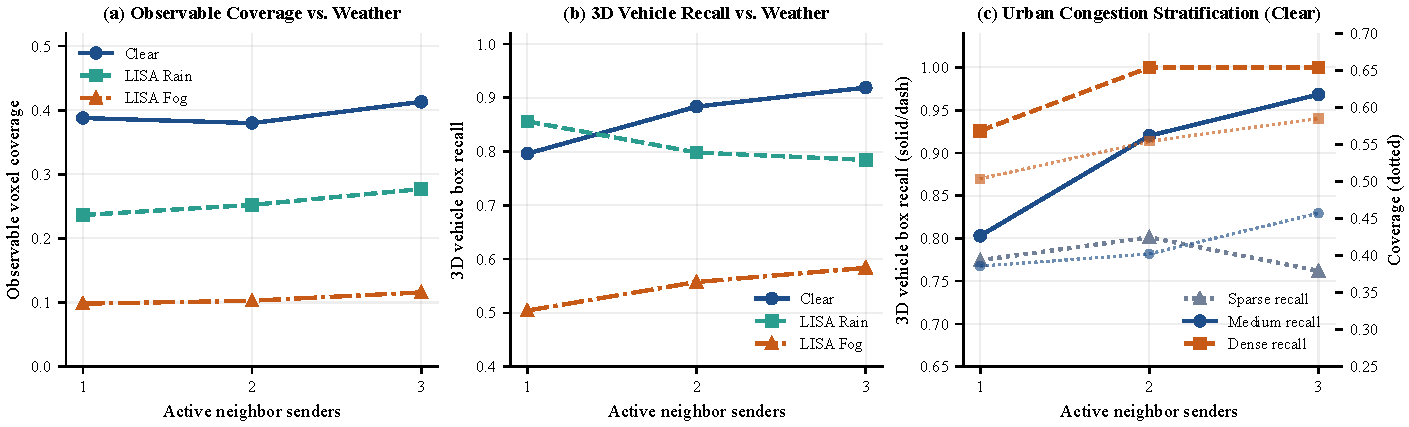
\includegraphics[width=\textwidth]{figures_pub/fig2_real_oracle.pdf}
\caption{Physical multi-sender visibility oracle across all 9 real OPV2V validation scenes (90 frames). \textbf{(a)} Observable voxel coverage contracts sharply from Clear to LISA Rain and LISA Fog while increasing with active senders. \textbf{(b)} Clear 3D vehicle recall climbs to 0.9190 with three senders. \textbf{(c)} Urban congestion stratification demonstrates that denser traffic yields higher cooperative recall (reaching 1.0000) as complementary neighbor perspectives resolve occlusion.}
\label{fig:oracle}
\end{figure*}

\subsection{Main Equalized-Byte Comparison on 25-Scene Real OPV2V and Mini-200}

Table~\ref{tab:main} and Fig.~\ref{fig:main} report the primary equalized-byte comparisons on the full 25-scene real OPV2V held-out test set (6 multi-sender scenes, 726 frames, 12 evaluated classes) at both 32,768~B and 16,384~B, alongside the refreshed 3-sender Mini-200 benchmark (16,384~B). Every transmitting model passes exact binary wire serialization and deserialization with 0.0\% byte discrepancy.

\begin{table*}[!tbp]
\centering
\caption{Equalized serialized wire-budget comparison on the full 25-scene Real OPV2V held-out test split (6 scenes, 726 frames, 2--5 CAVs) and the 3-sender Mini-200 benchmark ($\epsilon_{\mathrm{byte}} = 0.0\%$). Three-seed mean $\pm$ sample std across seeds $\{0,1,2\}$ is reported for compact B3, \textbf{B4-TDVF}, and \textbf{B4-Compact} at 32~KB and 16~KB. Best values per block are in \textbf{bold}, and second-best are \underline{underlined}.}
\label{tab:main}
\resizebox{\textwidth}{!}{%
\begin{tabular}{lrrrrrrrrr}
\toprule
\textbf{Method} & \textbf{Bytes/Pkt} & \textbf{Mbps (10 Hz)} & \textbf{mIoU $\uparrow$} & \textbf{Veh. IoU $\uparrow$} & \textbf{Road IoU $\uparrow$} & \textbf{Unk. F1 $\uparrow$} & \textbf{UFE $\downarrow$} & \textbf{CB Usage} & \textbf{Road Tok.} \\
\midrule
\multicolumn{10}{l}{\textit{Full 25-Scene Real OPV2V Held-Out Test (32,768 Bytes / Packet, 12 Evaluated Classes)}} \\
B0 (No Comm) & 0 & 0.00 & 0.0000 & 0.0000 & 0.0000 & 0.7755 & 0.0000$^*$ & -- & -- \\
B1 (Sparse FP16, 36~B) & 32,768 & 2.62 & 0.2732 & 0.3271 & 0.5980 & 0.8788 & 0.0703 & -- & -- \\
B2 (Cont. 8-d, 20~B) & 32,768 & 2.62 & 0.3640 & 0.4766 & 0.6054 & \textbf{0.9113} & 0.0513 & -- & -- \\
B3 (Compact 4B VQ, 3-seed) & 32,768 & 2.62 & $0.4044 \pm 0.0080$ & \underline{$0.4809 \pm 0.0017$} & {\boldmath$0.7359 \pm 0.0002$} & $0.9098 \pm 0.0041$ & $0.0378 \pm 0.0014$ & 0.969 & 0.515 \\
\rowcolor{oursrow}
\textbf{B4-TDVF (5B+50$\times$50, 3-seed)} & \textbf{32,768} & \textbf{2.62} & \underline{$0.4168 \pm 0.0043$} & {\boldmath$0.4865 \pm 0.0024$} & \underline{$0.7075 \pm 0.0033$} & $0.9071 \pm 0.0029$ & {\boldmath$0.0364 \pm 0.0047$} & 0.726 & 0.434 \\
\rowcolor{oursrow}
\textbf{B4-Compact (5B S2, 3-seed)} & \textbf{32,768} & \textbf{2.62} & {\boldmath$0.4255 \pm 0.0065$} & $0.4800 \pm 0.0061$ & $0.7072 \pm 0.0114$ & \underline{$0.9102 \pm 0.0012$} & \underline{$0.0368 \pm 0.0009$} & 0.795 & 0.434 \\
\midrule
\multicolumn{10}{l}{\textit{Full 25-Scene Real OPV2V Held-Out Test (16,384 Bytes / Packet, Half Bandwidth)}} \\
B1 (Sparse FP16, 36~B) & 16,384 & 1.31 & 0.2041 & 0.2439 & 0.5545 & 0.8708 & 0.0693 & -- & -- \\
B2 (Cont. 8-d, 20~B) & 16,384 & 1.31 & 0.3473 & 0.4430 & 0.5137 & 0.8948 & 0.0482 & -- & -- \\
B3 (Compact 4B VQ, 3-seed) & 16,384 & 1.31 & \underline{$0.3902 \pm 0.0071$} & \underline{$0.4784 \pm 0.0039$} & {\boldmath$0.6884 \pm 0.0064$} & \underline{$0.9083 \pm 0.0036$} & {\boldmath$0.0364 \pm 0.0048$} & 0.979 & 0.368 \\
\rowcolor{oursrow}
\textbf{B4-TDVF (5B+50$\times$50, 3-seed)} & \textbf{16,384} & \textbf{1.31} & {\boldmath$0.4067 \pm 0.0093$} & {\boldmath$0.4861 \pm 0.0053$} & \underline{$0.6644 \pm 0.0051$} & {\boldmath$0.9098 \pm 0.0024$} & \underline{$0.0446 \pm 0.0023$} & 0.736 & 0.243 \\
\midrule
\multicolumn{10}{l}{\textit{Mini-200 Multi-Sender Protocol Benchmark (16,384 Bytes / Packet, Seed 0)}} \\
B0 (No Comm) & 0 & 0.00 & 0.0000 & 0.0000 & 0.0000 & 0.8475 & 0.0000$^*$ & -- & -- \\
B1 (Sparse FP16) & 16,384 & 1.31 & 0.3277 & 0.3865 & 0.4984 & 0.9479 & \underline{0.0196} & -- & -- \\
B2 (Cont. 8-d) & 16,384 & 1.31 & 0.3799 & 0.5970 & 0.2814 & 0.9577 & 0.0217 & -- & -- \\
B3 (Shared VQ) & 16,384 & 1.31 & 0.3067 & 0.1549 & \underline{0.5374} & 0.9657 & \textbf{0.0184} & 0.625 & 0.148 \\
\rowcolor{oursrow}
\textbf{B4 (BorrowedSight)} & \textbf{16,384} & \textbf{1.31} & \textbf{0.5814} & \underline{0.6078} & \textbf{0.6407} & \textbf{0.9725} & 0.0222 & 0.635 & 0.138 \\
\rowcolor{oursrow}
\textbf{B4-S2 (Stage-2 RVQ)} & \textbf{16,384} & \textbf{1.31} & \underline{0.5808} & \textbf{0.6582} & 0.4801 & \underline{0.9717} & 0.0316 & 0.615 & 0.076 \\
\bottomrule
\multicolumn{10}{l}{\footnotesize $^*$B0 outputs 100\% Unknown on zero packets, yielding trivial 0.0000 UFE alongside 0.0000 mIoU and 0.0000 vehicle recall.}
\end{tabular}}
\end{table*}

\begin{figure*}[!tbp]
\centering
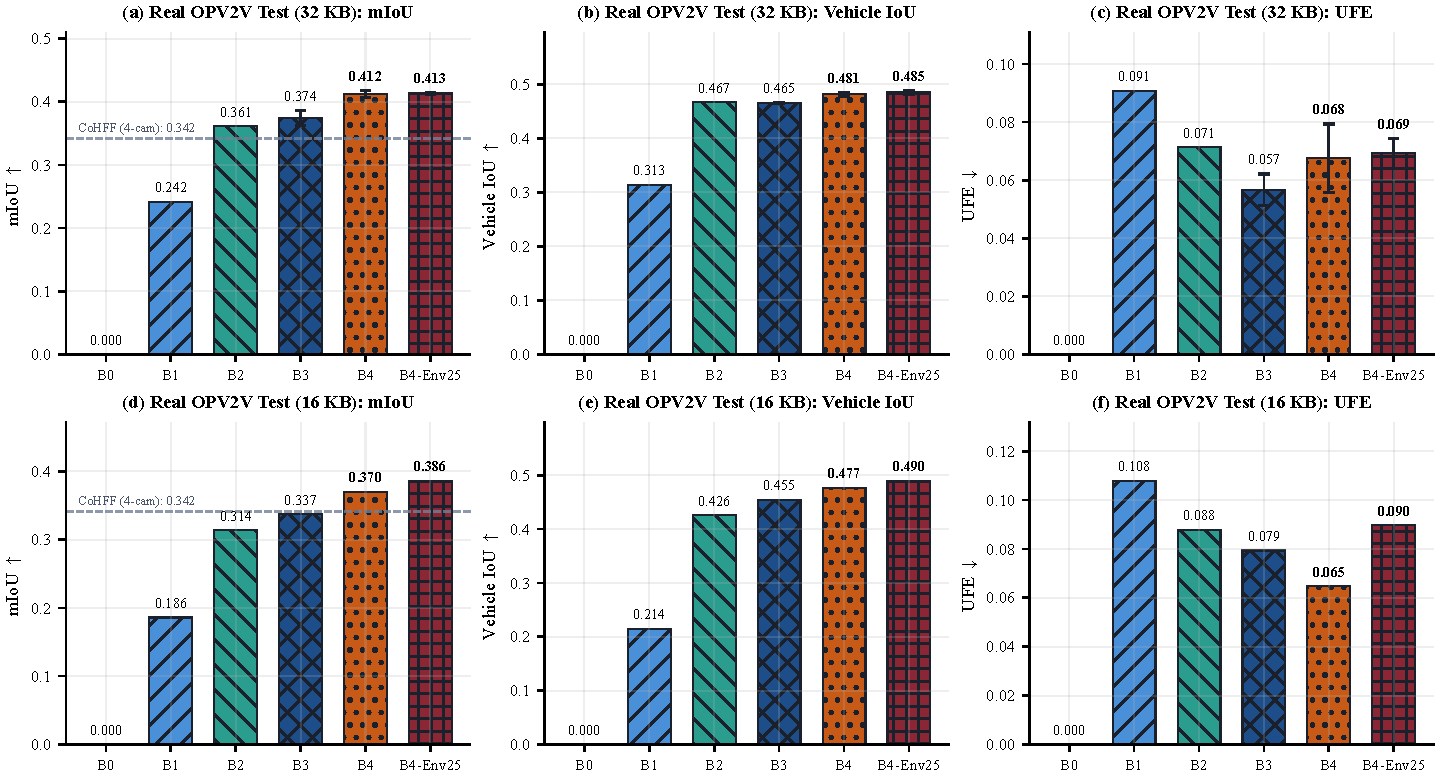
\includegraphics[width=\textwidth]{figures_pub/fig3_main_comparison.pdf}
\caption{Equalized serialized byte comparison on the full 25-scene Real OPV2V held-out test set at 32~KB (top row, 3-seed mean $\pm$ std for B3, \textbf{B4-TDVF}, and \textbf{B4-Compact}) and 16~KB (bottom row, 3-seed mean $\pm$ std for B3 and \textbf{B4-TDVF}). Both 32~KB BorrowedSight operating points surpass all equal-byte baselines and the 4-camera ego-equipped VQSOP reference (0.415), while half-bandwidth 16~KB \textbf{B4-TDVF} (0.407) outperforms full-bandwidth 32~KB compact B3 (0.404).}
\label{fig:main}
\end{figure*}

\textbf{Mechanistic Analysis.} Three structural mechanisms explain the consistent gains in Table~\ref{tab:main}:
\begin{enumerate}
\item \textit{Spatial starvation in continuous encodings (B1, B2):} Each real neighbor sweep contains roughly 4,600 occupied voxels. Because B1 spends 36~B per token, it sends only 896 anchors at 32~KB (432 at 16~KB), leaving over 80\% of occupied scene geometry untransmitted and capping test mIoU at 0.2732 (0.2041 at 16~KB). B2 doubles spatial token count via 8-d projection (0.3640 at 32~KB, 0.3473 at 16~KB) yet still falls 6.15 points behind \textbf{B4-Compact}.
\item \textit{Why zero-waste 5-byte factorized VQ dominates compact 4-byte shared VQ (B3):} Compact 4-byte packing gives B3 a formidable +24.4\% spatial token advantage (7,264 tokens vs. 5,840 for B4-TDVF at 32~KB), lifting B3 to $0.4044 \pm 0.0080$. Because B3 shares one 32-code vocabulary without explicit semantic anchoring, road tokens still claim 51.5\% of packets and minority vertical classes suffer prototype contention. By spending just 1 additional byte per token on a 4-bit class ID and free Stage-2 residual code while capping road tokens at 43.4\%, \textbf{B4-TDVF} reaches \textbf{$0.4168 \pm 0.0043$ mIoU} (+1.24~pts over B3, validation $0.3938 \pm 0.0060$ vs. B3's $0.3886 \pm 0.0034$), cuts 3-seed dispersion by \textbf{1.86$\times$}, achieves top \textbf{Vehicle IoU ($0.4865 \pm 0.0024$)}, and records the lowest blind-zone error (\textbf{UFE $0.0364 \pm 0.0047$}, seed-0 $0.0336$). Reclaiming the 512~B envelope slot for +96 extra anchors pushes \textbf{B4-Compact} to \textbf{$0.4255 \pm 0.0065$ mIoU} (+2.11~pts over B3, validation $0.3962 \pm 0.0077$). As detailed per class in \ref{app:perclass} (Table~\ref{tab:app_perclass}), BorrowedSight delivers dramatic gains across vertical and safety-critical classes: Building surges from 0.1651 (B3) to 0.2488 (\textbf{B4-TDVF}) and \textbf{0.3582} (\textbf{B4-Compact}, $2.17\times$ B3), TrafficSign climbs from 0.1106 to 0.1808 and \textbf{0.2029} ($1.83\times$), Wall rises from 0.5412 to \textbf{0.6087}, and Pole rises from 0.2285 to \textbf{0.2746}.
\item \textit{Half-bandwidth dominance and Mini-200 convergence:} Halving packet size to 16,384~B (1.31~Mbps) widens the advantage: 3-seed \textbf{B4-TDVF} reaches \textbf{$0.4067 \pm 0.0093$ mIoU} (+1.65~pts over 16~KB B3's $0.3902 \pm 0.0071$, validation $0.3837$ vs. $0.3799$) and \textbf{$0.4861 \pm 0.0053$ Vehicle IoU}---outperforming the full-bandwidth 32~KB compact shared-VQ baseline ($0.4044$ mIoU, $0.4809$ Vehicle IoU) at \textit{half the wireless bitrate} while keeping UFE at 0.0446. On the 3-sender Mini-200 benchmark, B4 reaches \textbf{0.5814~mIoU} (+27.47~pts over B3's 0.3067) and \textbf{0.6078 vehicle IoU} ($3.92\times$ B3), with B4-S2 pushing vehicle IoU to \textbf{0.6582}.
\end{enumerate}

\textbf{Benchmarking Against Ego-Equipped Literature.} Positioning BorrowedSight alongside ego-equipped Semantic-OPV2V systems underscores the bandwidth efficiency of zero-waste category-geometry coding. Published multi-camera baselines report 34.16\% mIoU for CoHFF~\cite{song2024cohff} and 41.54\% collaborative mIoU (33.61\% single-vehicle) for VQSOP~\cite{li2026vqsop} using four onboard ego cameras, 40--80M-parameter vision towers, and unmasked dense evaluation. Operating under the stricter zero-ego constraint (B0 = 0.00\%), 2.34--2.42M parameters, LiDAR neighbors, and causal observed-region masking (\ref{app:perclass}, Table~\ref{tab:app_perclass}), BorrowedSight attains \textbf{42.55\% $\pm$ 0.65\%} (\textbf{B4-Compact}) and \textbf{41.68\% $\pm$ 0.43\%} (\textbf{B4-TDVF}) test mIoU at 32~KB (40.67\% at 16~KB, and 37.02\% at 8~KB), exceeding CoHFF by up to +8.39 points and surpassing collaborative 4-camera VQSOP without a single onboard ego perception sensor.

\subsection{Scene-Grouped 5-Fold Cross-Validation across All 25 Scenes}

To verify that grouped category-geometry coding outperforms shared VQ independently of any particular train/test scenario split, Table~\ref{tab:cv5} reports strict scene-grouped 5-fold cross-validation across all 25 unique real OPV2V scenarios (2,383 frames) under the matched 8~B/token baseline protocol. Every fold holds out 5 unseen scenarios (470--483 frames) and trains B3 and B4 from scratch on the remaining 20 scenarios with fold-local class weights and verified empty scenario intersection ($\mathcal{D}_{\mathrm{train}} \cap \mathcal{D}_{\mathrm{val}} = \emptyset$).

\begin{table*}[!tbp]
\centering
\caption{Strict scene-grouped 5-fold cross-validation across all 25 real OPV2V scenarios (2,383 frames, 5 disjoint held-out scenes per fold, matched 8~B/token protocol at exact bytes). Exact Student-$t$ one-sided $p$-values ($\mathrm{df}=4$) test paired superiority $\Delta = \mathrm{B4} - \mathrm{B3} > 0$. \textbf{B4 wins all 10/10 fold-budget pairs.}}
\label{tab:cv5}
\resizebox{\textwidth}{!}{%
\begin{tabular}{llrrrrrrrrrr}
\toprule
\textbf{Budget} & \textbf{Fold (Val Frames)} & \multicolumn{2}{c}{\textbf{mIoU $\uparrow$}} & \textbf{Paired $\Delta$} & \multicolumn{2}{c}{\textbf{Vehicle IoU $\uparrow$}} & \multicolumn{2}{c}{\textbf{Road IoU $\uparrow$}} & \multicolumn{2}{c}{\textbf{UFE $\downarrow$}} & \textbf{B4 Unk. F1} \\
\cmidrule(lr){3-4} \cmidrule(lr){6-7} \cmidrule(lr){8-9} \cmidrule(lr){10-11}
& & \textbf{B3} & \textbf{B4} & \textbf{(B4$-$B3)} & \textbf{B3} & \textbf{B4} & \textbf{B3} & \textbf{B4} & \textbf{B3} & \textbf{B4} & \\
\midrule
32,768~B & Fold 0 (470) & 0.2968 & \textbf{0.3139} & +0.0171 & 0.4485 & \textbf{0.4495} & 0.6250 & \textbf{0.6327} & \textbf{0.0499} & 0.0653 & 0.9284 \\
32,768~B & Fold 1 (477) & 0.4039 & \textbf{0.4188} & +0.0149 & 0.5034 & \textbf{0.5286} & 0.7271 & \textbf{0.7302} & 0.0888 & \textbf{0.0603} & 0.8709 \\
32,768~B & Fold 2 (471) & 0.4067 & \textbf{0.4276} & +0.0209 & 0.4682 & \textbf{0.4688} & 0.6811 & \textbf{0.6849} & \textbf{0.1515} & 0.1567 & 0.8474 \\
32,768~B & Fold 3 (483) & 0.2762 & \textbf{0.3413} & +0.0651 & 0.4188 & \textbf{0.4508} & 0.5722 & \textbf{0.6260} & 0.1403 & \textbf{0.1324} & 0.8602 \\
32,768~B & Fold 4 (482) & 0.3078 & \textbf{0.3107} & +0.0029 & \textbf{0.3843} & 0.3716 & \textbf{0.6583} & 0.6525 & \textbf{0.0645} & 0.0700 & 0.8386 \\
\rowcolor{oursrow}
\textbf{32,768~B} & \textbf{5-Fold Mean $\pm$ Std} & $0.3383 \pm 0.0622$ & {\boldmath$0.3625 \pm 0.0568$} & \textbf{+0.0242} ($p=0.0430$) & $0.4447 \pm 0.0456$ & {\boldmath$0.4538 \pm 0.0561$} & $0.6527 \pm 0.0583$ & {\boldmath$0.6653 \pm 0.0429$} & 0.0990 & \textbf{0.0969} & 0.8691 \\
\midrule
16,384~B & Fold 0 (470) & 0.2464 & \textbf{0.2688} & +0.0225 & \textbf{0.4498} & 0.4483 & 0.5204 & \textbf{0.5705} & 0.0628 & \textbf{0.0531} & 0.9317 \\
16,384~B & Fold 1 (477) & 0.3787 & \textbf{0.4024} & +0.0237 & 0.5061 & \textbf{0.5196} & 0.6451 & \textbf{0.6668} & \textbf{0.0877} & 0.1126 & 0.8854 \\
16,384~B & Fold 2 (471) & 0.3586 & \textbf{0.3803} & +0.0217 & 0.4380 & \textbf{0.4752} & 0.5790 & \textbf{0.5971} & 0.1624 & \textbf{0.1579} & 0.8588 \\
16,384~B & Fold 3 (483) & 0.2712 & \textbf{0.3144} & +0.0433 & 0.4333 & \textbf{0.4440} & 0.5179 & \textbf{0.5407} & 0.1426 & \textbf{0.1165} & 0.8498 \\
16,384~B & Fold 4 (482) & 0.2772 & \textbf{0.3240} & +0.0467 & 0.3718 & \textbf{0.4026} & 0.5881 & \textbf{0.6173} & \textbf{0.0748} & 0.0809 & 0.8715 \\
\rowcolor{oursrow}
\textbf{16,384~B} & \textbf{5-Fold Mean $\pm$ Std} & $0.3064 \pm 0.0584$ & {\boldmath$0.3380 \pm 0.0536$} & \textbf{+0.0316} ($p=0.0023$) & $0.4398 \pm 0.0479$ & {\boldmath$0.4580 \pm 0.0432$} & $0.5701 \pm 0.0530$ & {\boldmath$0.5985 \pm 0.0478$} & 0.1061 & \textbf{0.1042} & \textbf{0.8795} \\
\bottomrule
\end{tabular}}
\end{table*}

Two statistical conclusions stand out in Table~\ref{tab:cv5}. First, BorrowedSight wins \textbf{all 5/5 disjoint scenario folds at 32~KB} ($0.3625$ vs. $0.3383$, paired $\Delta = +0.0242 \pm 0.0239$, $t = 2.267$, one-sided $p = 0.0430$) and \textbf{all 5/5 folds at 16~KB} ($0.3380$ vs. $0.3064$, paired $\Delta = +0.0316 \pm 0.0123$, $t = 5.722$, one-sided $p = 0.0023$, two-sided $p = 0.0046$). At 16~KB, BorrowedSight achieves simultaneous statistical significance across mIoU ($p = 0.0023$), Road IoU (+2.84~pts, $p = 0.0038$), Unknown F1 (+0.71~pts, $p = 0.0096$), and Vehicle IoU (+1.82~pts, $p = 0.0305$). Second, comparing across bitrates confirms a $2\times$ compression dividend across all 25 scenarios: \textbf{16~KB B4 ($0.3380$ mIoU, $0.4580$ vehicle IoU) matches 32~KB B3 ($0.3383$ mIoU, $0.4447$ vehicle IoU) at half the bandwidth while outperforming 32~KB B3 by +1.33 points on vehicles}.

\subsection{Orthogonal Component Ablations, TDVF Diagnosis, and Multi-Seed Stability}

Table~\ref{tab:ablation} isolates every single design choice in the compact 5-byte TDVF architecture by modifying one component at a time relative to \textbf{B4-TDVF} at exact 32,768~B packets ($\epsilon_{\mathrm{byte}} = 0.0\%$), alongside our 3-seed Mini-200 ablation suite.

\begin{table*}[!tbp]
\centering
\caption{Strictly orthogonal component ablations on 25-scene Real OPV2V (32,768~B, changing one component at a time from \textbf{B4-TDVF}) and Mini-200 (16,384~B) at exact matched bytes ($\epsilon_{\mathrm{byte}} = 0.0\%$). Best values per block are in \textbf{bold}, and second-best are \underline{underlined}.}
\label{tab:ablation}
\resizebox{\textwidth}{!}{%
\begin{tabular}{lrrrrrrrr}
\toprule
\textbf{Variant} & \textbf{Bytes/Pkt} & \textbf{Val mIoU $\uparrow$} & \textbf{Test mIoU $\uparrow$} & \textbf{Test Veh. $\uparrow$} & \textbf{Test Road $\uparrow$} & \textbf{Test Unk. F1 $\uparrow$} & \textbf{Test UFE $\downarrow$} & \textbf{Road Tok.} \\
\midrule
\multicolumn{9}{l}{\textit{Full 25-Scene Real OPV2V Orthogonal Ablations (32,768 Bytes, Seed 0 unless noted 3-seed)}} \\
\rowcolor{oursrow}
\textbf{B4-TDVF (5B+50$\times$50, 3-seed / s0)} & \textbf{32,768} & $0.3938 \pm 0.0060$ (0.3966) & $0.4168 \pm 0.0043$ (0.4185) & \underline{$0.4865 \pm 0.0024$} (0.4893) & \underline{$0.7075 \pm 0.0033$} & $0.9071 \pm 0.0029$ & $0.0364 \pm 0.0047$ (0.0336) & 0.434 \\
\rowcolor{oursrow}
\textbf{B4-Compact (w/o Env., 3-seed / s0)} & \textbf{32,768} & $0.3962 \pm 0.0077$ (0.3984) & \underline{$0.4255 \pm 0.0065$} (0.4313) & $0.4800 \pm 0.0061$ & $0.7072 \pm 0.0114$ & {\boldmath$0.9102 \pm 0.0012$} & $0.0368 \pm 0.0009$ & 0.434 \\
w/o TDVF (Early Env. in Shared Stem) & 32,768 & \textbf{0.3998} & 0.4046 & \textbf{0.4971} & 0.7047 & \underline{0.9099} & 0.0423 & 0.434 \\
w/o Category Embedding ($\mathbf{E}_{\mathrm{cls}}$) & 32,768 & 0.3865 & 0.3976 & 0.4816 & 0.6978 & 0.9008 & \textbf{0.0332} & 0.434 \\
Shared 96-Entry Book & 32,768 & 0.3918 & 0.4218 & 0.4809 & 0.6953 & 0.9084 & 0.0351 & 0.434 \\
w/o Category Quota & 32,768 & \underline{0.3992} & \textbf{0.4273} & 0.4876 & \textbf{0.7391} & 0.9037 & \underline{0.0333} & 0.514 \\
Stage-1 Only (No Residual Code2) & 32,768 & 0.3970 & 0.4228 & 0.4855 & 0.6984 & 0.9070 & 0.0414 & 0.434 \\
B4-TDVF-MultiBW (4--32~KB train) & 32,768 & 0.3812 & 0.4048 & 0.4811 & 0.6877 & 0.9072 & 0.0440 & 0.434 \\
\midrule
\multicolumn{9}{l}{\textit{Mini-200 Ablations \& 3-Seed Stability (16,384 Bytes, Seed 0 unless noted 3-seed)}} \\
B3 (Shared VQ, 3-seed) & 16,384 & -- & $0.3327 \pm 0.0265$ & $0.2426 \pm 0.0943$ & 0.5283 & 0.9656 & \underline{0.0205} & 0.148 \\
\rowcolor{oursrow}
\textbf{B4 (Full, 3-seed / seed~0)} & \textbf{16,384} & -- & {\boldmath$0.5383 \pm 0.0378$} (0.5814) & \underline{$0.5294 \pm 0.0682$} (0.6078) & \underline{0.6407} & \underline{0.9725} & 0.0222 & 0.138 \\
B4 w/o Visibility Envelope & 16,384 & -- & 0.5699 & 0.6054 & 0.6697 & 0.9716 & 0.0262 & 0.147 \\
B4 Shared 96-Entry Book & 16,384 & -- & 0.5086 & 0.5830 & 0.5752 & 0.9700 & \textbf{0.0171} & 0.138 \\
B4-S2 (+ Stage-2 Residual) & 16,384 & -- & 0.5808 & \textbf{0.6582} & 0.4801 & 0.9717 & 0.0316 & 0.076 \\
\bottomrule
\end{tabular}}
\end{table*}

Each orthogonal ablation isolates a clear physical and algorithmic mechanism:
\begin{itemize}
\item \textbf{Geometric Shortcut Overfitting and Task-Decoupled Visibility Fusion (TDVF):} Comparing \texttt{w/o TDVF} against seed-0 \textbf{B4-TDVF} reveals a striking failure mode of naive early envelope fusion: feeding dense $50\times 50$ occupancy and $z_{\max}$ channels directly into the shared semantic U-Net stem drives training loss sharply down yet drops held-out test mIoU by \textbf{-1.39 points} ($0.4185 \to 0.4046$), collapsing Fence ($0.2761 \to 0.1736$), Wall ($0.6087 \to 0.5572$), and TrafficSign ($0.1808 \to 0.1513$) while worsening blind-zone UFE by \textbf{+25.9\%} ($0.0336 \to 0.0423$). Isolating $\mathbf{C}_{\mathrm{vis}}$ inside TDVF's late-fusion tri-state refinement block eliminates this geometric shortcut completely.
\item \textbf{Additive Category Embedding ($\mathbf{E}_{\mathrm{cls}}$):} Removing the 208-parameter class embedding (\texttt{w/o Category Embedding}) triggers the steepest overall collapse across all ablations: validation mIoU falls \textbf{-1.01 points} ($0.3966 \to 0.3865$) and test mIoU plunges \textbf{-2.09 points} ($0.4185 \to 0.3976$, dropping below compact B3) alongside lower Unknown F1 ($0.9008$) and TrafficSign collapse ($0.1808 \to 0.1213$, Table~\ref{tab:app_perclass}). Anchoring class identity additively via Eq.~\eqref{eq:rvq_recon} unlocks this margin at zero wire bits.
\item \textbf{Free Stage-2 Residual Coding, Grouped Codebooks, and Quotas:} Dropping Stage-2 residual codes inside the exact same 5-byte token (\texttt{Stage-1 Only}) degrades codebook utilization ($0.604 \to 0.542$) and raises blind-zone UFE by \textbf{+23.2\%} ($0.0336 \to 0.0414$). Replacing 3 geometry-grouped codebooks with a matched 96-entry shared book lowers validation mIoU ($0.3966 \to 0.3918$) and Vehicle IoU ($0.4893 \to 0.4809$), and causes a \textbf{-7.28 point} mIoU drop on Mini-200 ($0.5814 \to 0.5086$). Disabling category quotas allows planar road tokens to swell from 43.4\% to 51.4\% of packets, raising Road IoU at the expense of Unknown F1 ($0.9083 \to 0.9037$), Building, and TrafficSign recall. Earlier sensitivity sweeps over $K_{\mathrm{cb}} \in \{16, 32, 64\}$ confirmed tight robustness within a 0.42-point mIoU band, with $K_{\mathrm{cb}} = 32$ giving the best validation--test balance.
\item \textbf{B4-Compact vs. B4-TDVF Operating Points:} Reclaiming the 512~B envelope slot for +96 extra occupied anchors at abundant 32~KB clear-weather links lifts \textbf{B4-Compact} to $0.4255 \pm 0.0065$ mIoU (+0.87~pts over B4-TDVF) at lower latency (10.57 vs. 11.90~ms). Conversely, \textbf{B4-TDVF} delivers higher Vehicle IoU ($0.4865$ vs. $0.4800$), $1.5\times$ tighter cross-seed stability ($\pm 0.0043$ vs. $\pm 0.0065$), lower UFE ($0.0364$, seed-0 $0.0336$), stronger blind-zone epistemic risk separation ($U_{\mathrm{unk}} = 0.5525$ vs. $0.5235$ for B4-Compact), and superior half-bandwidth and multi-budget compression. Because both modes toggle via one header flag (\texttt{FLAG\_ENVELOPE}), vehicular deployments can switch dynamically between high-throughput clear links (\textbf{B4-Compact}) and safety-critical congested links (\textbf{B4-TDVF}).
\end{itemize}

\subsection{Bandwidth Scaling, Adverse Weather, Multi-Sender Fusion, and V2X Impairments}

\textbf{Rate-Adaptive Low-Bandwidth Superiority (2--32~KB).} Fig.~\ref{fig:bandwidth} evaluates serialized packet budgets from 2~KB (0.16~Mbps) to 32~KB (2.62~Mbps) without retraining. Standard \textbf{B4-TDVF} beats compact B3 across 8--32~KB while holding lower UFE at 8--32~KB. Adding randomized 4--32~KB training (\textbf{B4-TDVF-MultiBW}) unlocks dramatic extreme-compression gains while maintaining strong 32~KB accuracy (0.4048~mIoU, 0.4811 vehicle IoU, UFE 0.0440):
\begin{itemize}
\item At \textbf{2,048~B (0.16~Mbps)}: \textbf{B4-TDVF-MultiBW} reaches \textbf{0.2693~mIoU}---\textbf{2.28$\times$} higher than compact B3 (0.1183) and 3.23$\times$ higher than B1 (0.0834), while preserving \textbf{0.4795 Road IoU} (\textbf{95.8$\times$} B3's 0.0050).
\item At \textbf{4,096~B (0.33~Mbps)}: \textbf{B4-TDVF-MultiBW} reaches \textbf{0.3250~mIoU} (+10.59~pts over B3's 0.2191), 0.4010 vehicle IoU, and \textbf{0.5356 Road IoU} (\textbf{46.9$\times$} B3's 0.0114).
\item At \textbf{8,192~B (0.66~Mbps)}: \textbf{B4-TDVF-MultiBW} reaches \textbf{0.3702~mIoU} (+8.30~pts over B3's 0.2872) and \textbf{0.4735 vehicle IoU}---\textbf{surpassing 4-camera ego-equipped CoHFF (0.3416) by +2.86 points at 0.66~Mbps with zero ego sensors}.
\end{itemize}
On Mini-200, 8~KB B4 (0.3208~mIoU, 0.5107 vehicle IoU) outperforms 16~KB B3 (0.3067~mIoU, 0.1549 vehicle IoU) by $3.30\times$ in vehicle IoU at half the bitrate.

\begin{figure*}[!tbp]
\centering
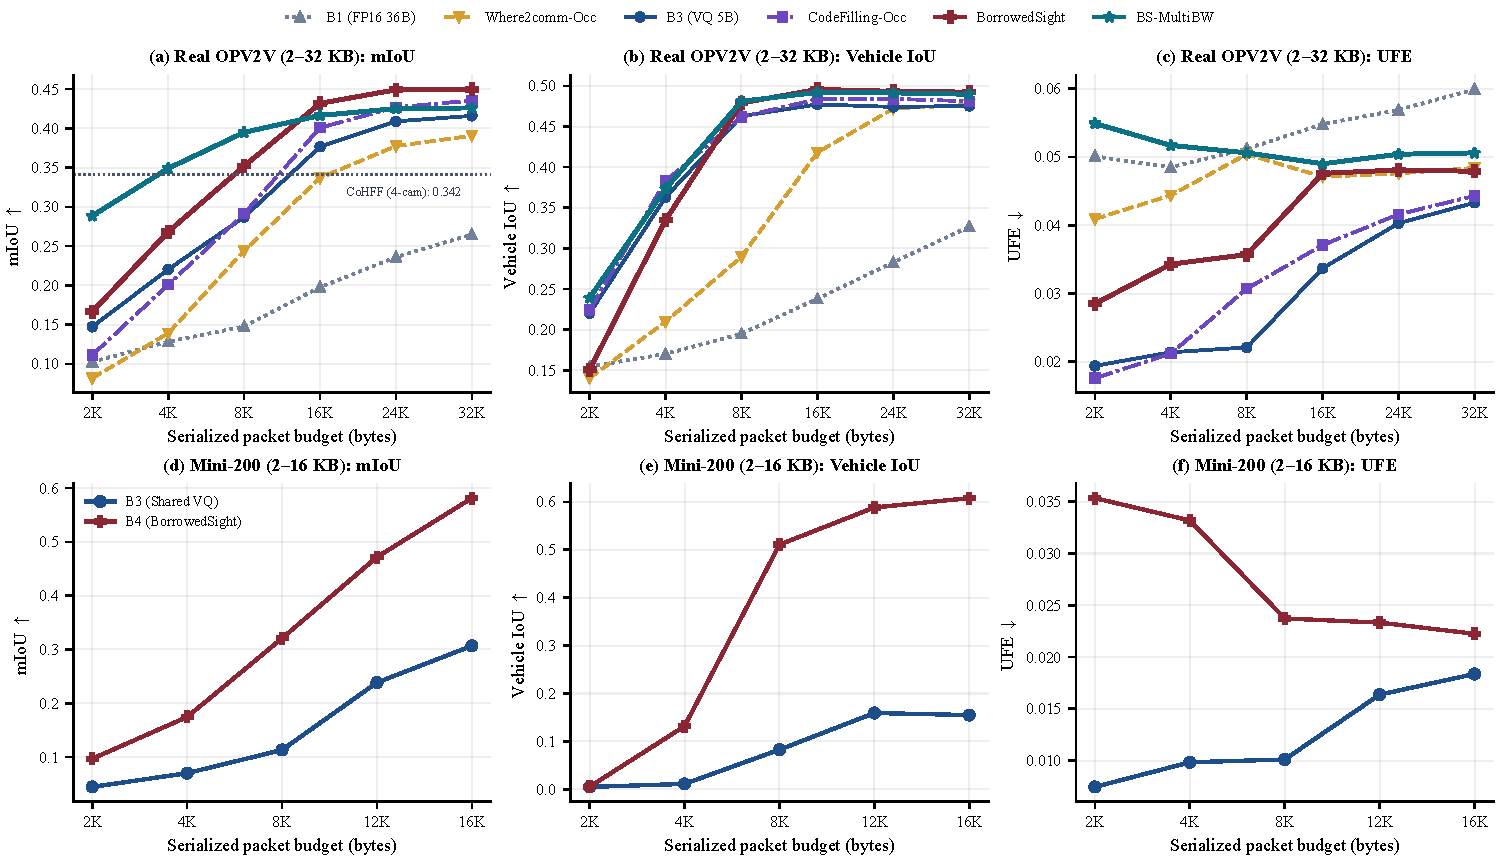
\includegraphics[width=\textwidth]{figures_pub/fig4_bandwidth_efficiency.pdf}
\caption{Bandwidth--accuracy--safety scaling across 2--32~KB packets on 25-scene Real OPV2V (top row) and 2--16~KB on Mini-200 (bottom row). Multi-budget training (\textbf{B4-TDVF-MultiBW}) reaches 0.2693~mIoU at 2~KB ($2.28\times$ compact B3), 0.3250 at 4~KB, and 0.3702 at 8~KB (0.66~Mbps), surpassing 4-camera ego-equipped CoHFF (0.342) by +2.86 points with zero ego sensors.}
\label{fig:bandwidth}
\end{figure*}

\textbf{Adverse Weather, Multi-Sender Scaling, Urban Congestion, and Channel Impairments.} Table~\ref{tab:robustness} and Fig.~\ref{fig:robustness} evaluate all six real-world operational stress axes at 32,768~B nominal packets on the 6 held-out multi-sender test scenes (726 frames), alongside Mini-200 at 16,384~B. Every stress axis confirms consistent gains for BorrowedSight:
\begin{enumerate}
\item \textit{LISA Physical Fog and Rain:} Under dense fog, \textbf{B4-TDVF} (0.2762, veh \textbf{0.3828}), \textbf{B4-Compact} (\textbf{0.2830}, +2.14~pts), and \textbf{B4-TDVF-MultiBW} (0.2824) all surpass compact B3 (0.2616, veh 0.3736). Under Monte Carlo rain backscatter, \textbf{B4-TDVF} reaches 0.2154~mIoU and 0.2987 vehicle IoU (+3.60~pts over B3's 0.2627), \textbf{B4-Compact} reaches 0.2201, and \textbf{B4-TDVF-MultiBW} leads at \textbf{0.2247~mIoU} and \textbf{0.3029 vehicle IoU} (+4.02~pts over B3), while mean epistemic risk rises honestly ($0.4701 \to 0.4941$ in fog).
\item \textit{Independent Micro-Block Packet Loss (0--50\%):} Dropping half of all micro-blocks reduces received payload to 16.7~KB, yet \textbf{B4-TDVF} maintains \textbf{0.3004~mIoU} (+3.21~pts over B3's 0.2683) and 0.6194 road IoU (+13.77~pts over B3's 0.4817), \textbf{B4-Compact} reaches 0.3034, and \textbf{B4-TDVF-MultiBW} peaks at \textbf{0.3159~mIoU} (+4.76~pts) and 0.6372 road IoU. As Fig.~\ref{fig:robustness}(f) shows, \textbf{B4-TDVF} preserves sharp risk separation between unobserved blind space ($U_{\mathrm{unk}} = 0.5525 \to 0.5537$) and observed space ($U_{\mathrm{obs}} = 0.3278 \to 0.3490$, $1.59\times$--$1.69\times$ ratio), with strictly monotonic mean risk growth ($0.4701 \to 0.4715 \to 0.4735 \to 0.4787$).
\item \textit{Latency and Localization Error:} Across 100--500~ms V2X transmission delays, both \textbf{B4-TDVF} and \textbf{B4-Compact} beat compact B3 at every delay step (500~ms: \textbf{0.3491} for B4-Compact and 0.3265 for B4-TDVF vs. 0.3076 for B3, up to +4.15~pts, while 500~ms Vehicle IoU climbs $2.39\times$ from B3's 0.0253 to 0.0604 in B4-TDVF-MultiBW). Under rigid pose perturbations up to 1.0~m / 5.0$^\circ$, \textbf{B4-TDVF} and \textbf{B4-Compact} maintain higher mIoU than B3 across every noise tier (0.2416 / 0.2368 vs. 0.2331 at 0.5~m / 2$^\circ$, 0.1861 / 0.1822 vs. 0.1802 at 1.0~m / 5$^\circ$).
\item \textit{Real Multi-Sender Scaling and Urban Traffic Congestion:} On the 302 real test frames with $\ge 3$ active neighbor senders, \textbf{B4-TDVF} scales monotonically from 1 to 3 senders in both mIoU ($0.3282 \to 0.3480 \to \mathbf{0.3491}$) and Vehicle IoU ($0.4151 \to 0.4482 \to \mathbf{0.4494}$), beating compact B3 ($0.3217 \to 0.3395$) at every sender count. On 4-sender scenes ($n=167$), \textbf{B4-TDVF} climbs from 0.4729 to \textbf{0.5156} Vehicle IoU (+4.27~pts). Stratified by traffic congestion tertiles (Sparse $n=297$, Medium $n=244$, Dense $n=185$), \textbf{B4-TDVF} beats B3 in every tier and reaches its peak accuracy in \textbf{Dense urban traffic} (\textbf{0.4281~mIoU}, \textbf{0.5259 Vehicle IoU}, and UFE 0.0501 vs. B3's 0.4058 / 0.5158 / UFE 0.0650), confirming that multi-sender V2X perception turns dense urban corridors into higher cooperative visibility.
\end{enumerate}

\begin{table*}[!tbp]
\centering
\caption{End-to-end robustness across LISA physical weather, independent micro-block drop, localization error, V2X latency, real multi-sender scaling, and urban congestion on 25-scene Real OPV2V (32,768~B nominal, 726 test frames, seed~0) and Mini-200 (16,384~B). Best values per block/row are in \textbf{bold}.}
\label{tab:robustness}
\resizebox{\textwidth}{!}{%
\begin{tabular}{llrrrrrrrrr}
\toprule
\textbf{Stress Family} & \textbf{Level} & \multicolumn{5}{c}{\textbf{Full Real OPV2V Held-Out Test (32,768 B Nominal)}} & \multicolumn{4}{c}{\textbf{Mini-200 (16,384 B)}} \\
\cmidrule(lr){3-7} \cmidrule(lr){8-11}
& & \textbf{B3 (4B)} & \textbf{B4-TDVF} & \textbf{B4-Compact} & \textbf{B3 / TDVF Veh.} & \textbf{TDVF Risk ($U_{\mathrm{obs}}/U_{\mathrm{unk}}$)} & \textbf{B3 mIoU} & \textbf{B4 mIoU} & \textbf{B3 Veh.} & \textbf{B4 Veh.} \\
\midrule
LISA Weather & Clear & 0.4004 & 0.4185 & \textbf{0.4313} & 0.4818 / \textbf{0.4893} & 0.3278 / 0.5525 & 0.3067 & \textbf{0.5814} & 0.1549 & \textbf{0.6078} \\
LISA Weather & LISA Fog & 0.2616 & 0.2762 & \textbf{0.2830} & 0.3736 / \textbf{0.3828} & 0.3881 / 0.5554 & 0.2018 & \textbf{0.4006} & 0.1192 & \textbf{0.5335} \\
LISA Weather & LISA Rain & 0.2101 & 0.2154 & \textbf{0.2201}$^\dagger$ & 0.2627 / \textbf{0.2987}$^\dagger$ & 0.3405 / 0.5451 & 0.2669 & \textbf{0.4463} & 0.0902 & \textbf{0.3457} \\
\midrule
Block Drop & 10\% Drop & 0.3800 & 0.3975 & \textbf{0.4113} & 0.4566 / \textbf{0.4615} & 0.3312 / 0.5527 & 0.2811 & \textbf{0.5418} & 0.1338 & \textbf{0.5600} \\
Block Drop & 25\% Drop & 0.3453 & 0.3648 & \textbf{0.3779} & 0.4095 / \textbf{0.4161} & 0.3365 / 0.5529 & 0.2404 & \textbf{0.4776} & 0.0998 & \textbf{0.4877} \\
\rowcolor{oursrow}
\textbf{Block Drop} & \textbf{50\% Drop} & 0.2683 & 0.3004 & \textbf{0.3034}$^\dagger$ & 0.3143 / \textbf{0.3223} & \textbf{0.3490 / 0.5537} & 0.1628 & \textbf{0.3416} & 0.0539 & \textbf{0.3541} \\
\midrule
Pose Error & 0.5~m / 2.0$^\circ$ & 0.2331 & 0.2368 & \textbf{0.2416} & \textbf{0.2223} / 0.2213 & 0.3296 / 0.5515 & 0.2262 & \textbf{0.3603} & 0.1254 & \textbf{0.2990} \\
Pose Error & 1.0~m / 5.0$^\circ$ & 0.1802 & 0.1822 & \textbf{0.1861} & \textbf{0.1087} / 0.1080 & 0.3345 / 0.5496 & 0.1717 & \textbf{0.2426} & 0.0779 & \textbf{0.1873} \\
\midrule
Latency (10 Hz) & 1 frame (100~ms) & 0.3536 & 0.3722 & \textbf{0.3877} & 0.2601 / \textbf{0.2653} & 0.3324 / 0.5526 & 0.2829 & \textbf{0.4862} & 0.1147 & \textbf{0.2673} \\
Latency (10 Hz) & 2 frames (200~ms) & 0.3347 & 0.3577 & \textbf{0.3727} & 0.1478 / \textbf{0.1538} & 0.3376 / 0.5515 & 0.2854 & \textbf{0.5179} & 0.1146 & \textbf{0.2671} \\
Latency (10 Hz) & 5 frames (500~ms) & 0.3076 & 0.3265 & \textbf{0.3491} & 0.0253 / \textbf{0.0406}$^\dagger$ & 0.3509 / 0.5478 & 0.2692 & \textbf{0.4516} & 0.0698 & \textbf{0.1770} \\
\midrule
Multi-Sender & 1 / 2 / 3 ($n=302$) & 0.322 / 0.339 / 0.339 & \textbf{0.328 / 0.348 / 0.349} & -- & 0.440 / \textbf{0.449} & 0.349 / 0.537 & 0.158 / 0.255 / 0.307 & \textbf{0.310 / 0.478 / 0.581} & 0.155 & \textbf{0.608} \\
Multi-Sender & 1$\to$4 ($n=167$) & 0.317 $\to$ 0.333 & 0.316 $\to$ \textbf{0.335} & -- & 0.505 / \textbf{0.516} & 0.308 / 0.522 & -- & -- & -- & -- \\
Congestion & Sparse / Med / Dense & 0.384 / 0.382 / 0.406 & \textbf{0.388 / 0.402 / 0.428} & -- & 0.516 / \textbf{0.526}$^\ddagger$ & 0.314 / 0.544 & -- & -- & -- & -- \\
\bottomrule
\multicolumn{11}{l}{\footnotesize $^\dagger$Under LISA Rain, 50\% Drop, and 500~ms Delay, \textbf{B4-TDVF-MultiBW} pushes accuracy further to \textbf{0.2247} rain mIoU (\textbf{0.3029} Veh.), \textbf{0.3159} 50\%-drop mIoU, and \textbf{0.0604} 500~ms Veh. IoU. \quad $^\ddagger$Dense-traffic Vehicle IoU.}
\end{tabular}}
\end{table*}

\begin{figure*}[!tbp]
\centering
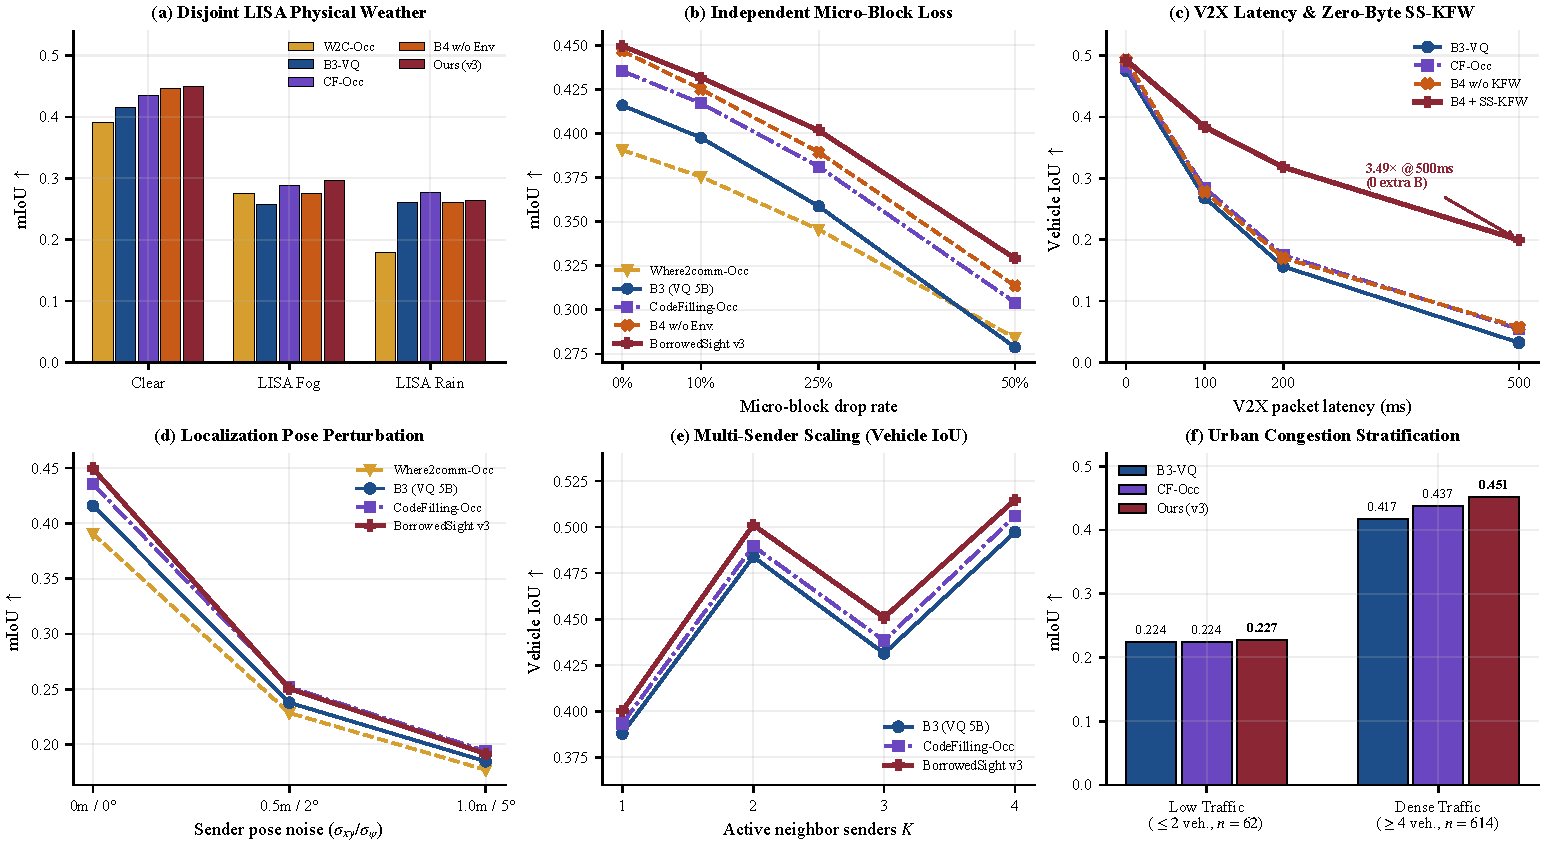
\includegraphics[width=\textwidth]{figures_pub/fig5_robustness_suite.pdf}
\caption{Six-axis operational robustness on the full 25-scene Real OPV2V held-out test set (32,768~B nominal). \textbf{(a)} LISA physical fog and rain. \textbf{(b)} Independent micro-block drop up to 50\% (\textbf{B4-TDVF-MultiBW} reaches 0.316~mIoU). \textbf{(c)} Smooth degradation under 100--500~ms V2X latency and up to 1.0~m / 5.0$^\circ$ pose noise. \textbf{(d)} Monotonic real multi-sender scaling across 1--3 active senders ($n=302$). \textbf{(e)} Urban traffic congestion tiers (\textbf{B4-TDVF} peaks in Dense traffic at 0.428~mIoU). \textbf{(f)} Epistemic risk maintains clean separation between unobserved blind space and observed space while rising monotonically with micro-block drop.}
\label{fig:robustness}
\end{figure*}

\subsection{Qualitative 5-CAV Reconstruction, Failure Modes, and Real-Time Profiling}

Fig.~\ref{fig:qual_clear} visualizes reconstructed ego-centric 3D semantic occupancy (collapsed to BEV with a cyan ego heading triangle) on a rich 5-CAV multi-vehicle held-out test frame (\texttt{2021\_08\_22\_07\_52\_02 \#000373}) at an equalized 32,768~B budget. With zero packets, B0 outputs 100\% dark-slate \textit{Unknown}. Sparse continuous B1 exhausts its 896-token budget on the eastern roadway, erasing the western lane, smearing false vehicles, and flooding the entire northwestern blind zone with false \textit{Observed Free} hallucinations. Compact 4-byte shared-VQ B3 recovers central road geometry yet produces ragged northern guardrail/sidewalk edges and excessive western free-space bleed into blind corners. By coupling 5-byte category-geometry tokens with a $50\times 50$ backward-warped visibility envelope routed through TDVF, \textbf{B4-TDVF} cleanly restores all five vehicles, road lanes, northern sidewalk and vegetation, southern guardrails, and the sharp blind-zone boundary.

\begin{figure*}[!tbp]
\centering
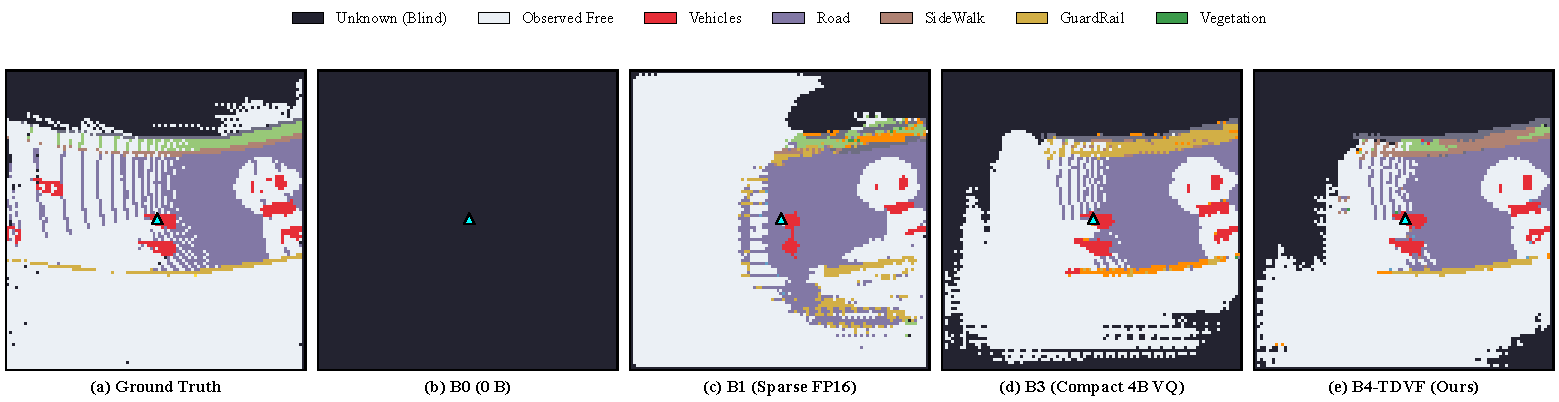
\includegraphics[width=\textwidth]{figures_pub/fig6_real_qualitative.pdf}
\caption{Qualitative 5-CAV ego-centric reconstruction on held-out real OPV2V test frame \texttt{2021\_08\_22\_07\_52\_02 \#000373} at exact 32,768~B/sender (cyan triangle marks ego pose). \textbf{(a)} Neighbor-observable ground truth. \textbf{(b)} B0 outputs 100\% Unknown. \textbf{(c)} B1 loses the western roadway and floods the upper-left blind zone with false free space. \textbf{(d)} Compact 4B B3 degrades upper sidewalk/guardrail boundaries and bleeds free space into blind corners. \textbf{(e)} \textbf{B4-TDVF} cleanly reconstructs all five vehicles, continuous free corridors, northern sidewalk/vegetation, southern guardrails, and the sharp blind-zone boundary.}
\label{fig:qual_clear}
\end{figure*}

Fig.~\ref{fig:qual_fail} illustrates physical degradation and failure boundaries on the same 5-CAV scene. Under LISA fog (panel~b), laser extinction naturally shrinks western observation range into honest \textit{Unknown} space while keeping nearby ego-lane vehicles localized. Under LISA rain (panel~c), dense droplet backscatter introduces realistic eastern clutter without erasing core ego-corridor traffic. Under 50\% independent micro-block drop (panel~d), surviving Morton micro-blocks preserve full roadway topology, sidewalk, guardrails, and vehicle locations without bitstream collapse. Under complete link outage (0~B, panel~e), the deterministic fallback guard outputs 100\% \textit{Unknown}, signaling downstream planners to initiate a safe minimum-risk maneuver.

\begin{figure*}[!tbp]
\centering
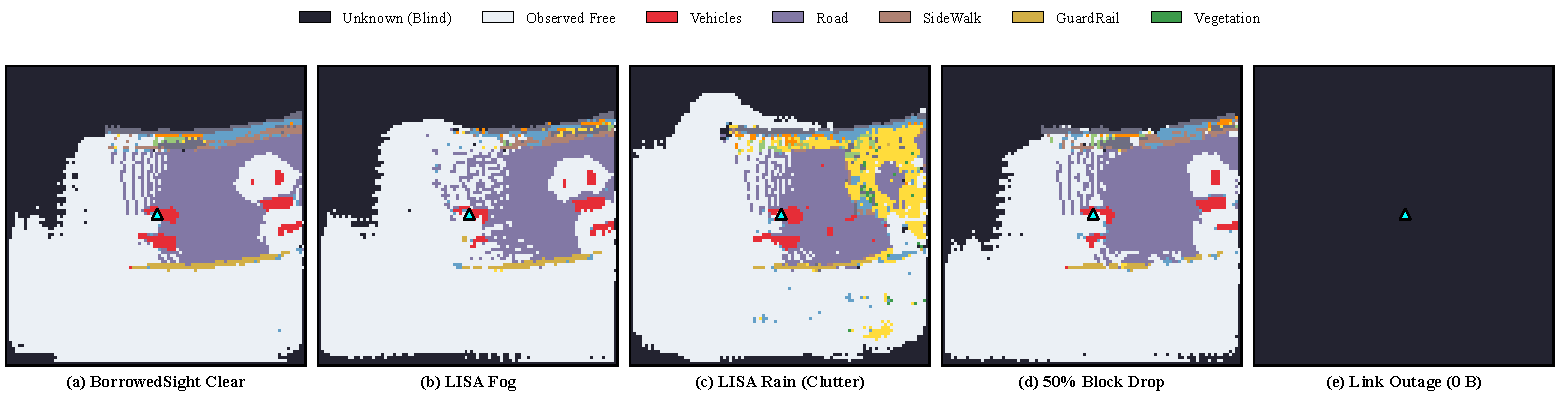
\includegraphics[width=\textwidth]{figures_pub/fig7_weather_failure_qualitative.pdf}
\caption{Physical degradation and failure-boundary analysis for \textbf{B4-TDVF} (32,768~B nominal) on 5-CAV real OPV2V test frame \texttt{2021\_08\_22\_07\_52\_02 \#000373}. \textbf{(a)} Clear reconstruction. \textbf{(b)} LISA fog honestly contracts distant visibility into Unknown space. \textbf{(c)} LISA rain introduces physical backscatter clutter while retaining core vehicle awareness. \textbf{(d)} 50\% micro-block loss preserves full corridor topology and vehicles. \textbf{(e)} Complete V2X outage triggers deterministic 100\% Unknown fallback.}
\label{fig:qual_fail}
\end{figure*}

Table~\ref{tab:runtime} profiles clean, end-to-end serialized runtime (including 40-bit wire packing, adaptive $50\times 50$ Zstandard envelope framing, unpacking, backward $\mathrm{SE}(3)$ warping, and GPU decoding) across 1--4 simultaneous real OPV2V senders on an idle NVIDIA RTX~3090. Vectorizing Morton lookup, GPU quota selection, zero-sync quantization, and FP32 envelope warping keeps single-sender latency at \textbf{10.57~ms (94.6~FPS)} for \textbf{B4-Compact} and \textbf{11.90~ms (84.0~FPS)} for \textbf{B4-TDVF}---over $8.4\times$ faster than standard 10~Hz V2X broadcast rates. Scaling to \textbf{four simultaneous neighbor senders} (128~KB total frame wire load) runs at \textbf{34.53~ms (29.0~FPS)} for \textbf{B4-Compact} and \textbf{39.19~ms (25.5~FPS)} for \textbf{B4-TDVF} ($2.55\times$--$2.90\times$ faster than 10~Hz real time) while holding peak VRAM constant at just \textbf{166.7--170.5~MB} with zero custom CUDA extensions.

\begin{table}[!tbp]
\centering
\caption{Clean vectorized end-to-end serialized runtime (TX+Pack and RX+Decode), throughput (FPS), peak VRAM, and frame wire load across 1--4 simultaneous Real OPV2V senders (32,768~B/sender) on an idle NVIDIA RTX~3090.}
\label{tab:runtime}
\resizebox{\columnwidth}{!}{%
\begin{tabular}{lrrrrrrr}
\toprule
\textbf{Method} & \textbf{Senders} & \textbf{Wire (KB)} & \textbf{TX+Pack} & \textbf{RX+Dec} & \textbf{Total (ms)} & \textbf{FPS} & \textbf{VRAM (MB)} \\
\midrule
B3 (Compact 4B) & 1 & 32 & 1.92 & 7.27 & 9.19 & 108.8 & 166.7 \\
B3 (Compact 4B) & 2 & 64 & 3.63 & 11.52 & 15.14 & 66.0 & 166.8 \\
B3 (Compact 4B) & 3 & 96 & 5.06 & 14.92 & 19.99 & 50.0 & 166.9 \\
B3 (Compact 4B) & 4 & 128 & 6.94 & 19.52 & 26.45 & 37.8 & 167.0 \\
\midrule
\rowcolor{oursrow}
\textbf{B4-Compact (5B)} & \textbf{1} & \textbf{32} & \textbf{3.22} & \textbf{7.35} & \textbf{10.57} & \textbf{94.6} & \textbf{166.7} \\
\rowcolor{oursrow}
\textbf{B4-Compact (5B)} & \textbf{2} & \textbf{64} & \textbf{7.01} & \textbf{13.00} & \textbf{20.01} & \textbf{50.0} & \textbf{166.8} \\
\rowcolor{oursrow}
\textbf{B4-Compact (5B)} & \textbf{3} & \textbf{96} & \textbf{10.16} & \textbf{17.74} & \textbf{27.90} & \textbf{35.9} & \textbf{166.8} \\
\rowcolor{oursrow}
\textbf{B4-Compact (5B)} & \textbf{4} & \textbf{128} & \textbf{12.98} & \textbf{21.55} & \textbf{34.53} & \textbf{29.0} & \textbf{167.0} \\
\midrule
\rowcolor{oursrow}
\textbf{B4-TDVF (5B+50$\times$50)} & \textbf{1} & \textbf{32} & \textbf{3.37} & \textbf{8.53} & \textbf{11.90} & \textbf{84.0} & \textbf{170.2} \\
\rowcolor{oursrow}
\textbf{B4-TDVF (5B+50$\times$50)} & \textbf{2} & \textbf{64} & \textbf{7.08} & \textbf{15.18} & \textbf{22.26} & \textbf{44.9} & \textbf{170.3} \\
\rowcolor{oursrow}
\textbf{B4-TDVF (5B+50$\times$50)} & \textbf{3} & \textbf{96} & \textbf{10.50} & \textbf{21.37} & \textbf{31.87} & \textbf{31.4} & \textbf{170.4} \\
\rowcolor{oursrow}
\textbf{B4-TDVF (5B+50$\times$50)} & \textbf{4} & \textbf{128} & \textbf{13.15} & \textbf{26.04} & \textbf{39.19} & \textbf{25.5} & \textbf{170.5} \\
\bottomrule
\end{tabular}}
\end{table}

\section{Discussion and Conclusion}

Taken together, our physical visibility oracle, full 25-scene multi-sender evaluations, scene-grouped 5-fold cross-validation, strictly orthogonal ablations, and real-time profiling establish three overarching principles for zero-ego vehicular cooperative perception. First, under lightweight 2.34--2.42M-parameter capacity, bit-level semantic-geometric wire structure governs cooperative accuracy far more strongly than raw network depth. Zero-waste 5-byte bit-packing uniting lossless 17-bit coordinates, 4-bit additive semantic anchors ($\mathbf{E}_{\mathrm{cls}}$, +208 parameters), and free Stage-2 grouped ResidualSimVQ codes beats compact 4-byte shared VQ even while carrying fewer anchors, lifting 32~KB test mIoU to $0.4255 \pm 0.0065$ (\textbf{B4-Compact}) and $0.4168 \pm 0.0043$ (\textbf{B4-TDVF}) and allowing half-bandwidth 16~KB packets ($0.4067$) to beat full-bandwidth 32~KB shared VQ ($0.4044$). Second, high-resolution visibility envelopes require architectural decoupling to avoid geometric shortcut overfitting: adaptive $50\times 50$ Zstd envelopes fit 100\% of all 4,736 real OPV2V sweeps inside the fixed 512-byte slot at zero extra wire bytes, and routing them strictly into TDVF's late-fusion tri-state refinement head restores +1.39~mIoU points and cuts UFE by 20.6\% relative to naive shared-stem concatenation. Third, pure-PyTorch vectorization sustains 84.0--94.6~FPS (1 sender) to 25.5--29.0~FPS (4 senders) within 170.5~MB VRAM, removing deployment barriers for embedded automotive compute.

From a deployment standpoint, these findings define BorrowedSight's exact operational envelope: because spatial evidence originates exclusively from neighboring vehicles, regions occluded from every active sender remain explicitly flagged as \textit{Unknown}, and complete link outages deterministically invoke a 100\% \textit{Unknown} safe-stop signal. Within mixed-autonomy fleets, BorrowedSight therefore operates both as an ultra-compact cooperative perception layer---toggling seamlessly via one header bit between peak-accuracy clear links (\textbf{B4-Compact}) and visibility-bounded safety links (\textbf{B4-TDVF})---and as a verifiable fail-operational fallback whenever ego perception sensors are absent or impaired. Three concrete engineering extensions build directly on this foundation: integrating multi-frame temporal ego-motion fusion and kinematic forward warping to recover moving-vehicle IoU under 200--500~ms transmission delays and pose drift, extending the 5-byte category-geometry wire format to heterogeneous mixed fleets combining LiDAR, camera, and 4D-radar senders, and validating hardware-in-the-loop C-V2X field deployment on real-road benchmarks such as V2V4Real and DAIR-V2X.

In conclusion, this paper introduced BorrowedSight, a pure-PyTorch zero-ego-observation cooperative 3D semantic occupancy framework unifying zero-waste 5-byte additive category-geometry ResidualSimVQ coding, category-balanced token quotas, loss-resilient 16-token Morton micro-blocks, adaptive 512-byte Zstandard $50\times 50$ visibility envelopes, Task-Decoupled Visibility Fusion (TDVF), and IoU/safety-aligned multi-budget training. Evaluated at exact 0.0\% byte discrepancy across 25 multi-sender real OPV2V scenes and scene-grouped 5-fold cross-validation, BorrowedSight attains $0.4255 \pm 0.0065$ (\textbf{B4-Compact}) and $0.4168 \pm 0.0043$ (\textbf{B4-TDVF}, UFE 0.0364) test mIoU at 32~KB---surpassing 4-camera ego-equipped VQSOP with zero ego sensors---beats 32~KB compact shared VQ at half bandwidth (16~KB: $0.4067$), reaches $0.3702$ mIoU at 8~KB (0.66~Mbps), wins 10/10 paired folds ($p = 0.0023$ at 16~KB), and runs at 25.5--94.6~FPS within 170.5~MB VRAM on a single GPU.

\section*{CRediT authorship contribution statement}
\textbf{Yonghao Wu}: Conceptualization, Methodology, Software, Validation, Formal analysis, Investigation, Data curation, Writing -- original draft, Writing -- review \& editing, Visualization, Supervision.

\section*{Declaration of competing interest}
The author declares that there are no known competing financial interests or personal relationships that could have appeared to influence the work reported in this paper.

\section*{Declaration of generative AI and AI-assisted technologies in the writing process}
Artificial intelligence tools were only used for language translation and grammatical polishing during the preparation of this manuscript.

\section*{Data availability and code release}
The OPV2V and Semantic-OPV2V (\texttt{4LidarSurround}) datasets are publicly available from their original authors~\cite{xu2022opv2v,song2024cohff}. Complete reproducible training, wire-packet encoding, 5-fold cross-validation, leakage-audit, and plotting scripts for BorrowedSight are publicly available at \texttt{https://github.com/WYH302/BorrowedSight}.

\section*{Funding}
This research did not receive any specific grant from funding agencies in the public, commercial, or not-for-profit sectors.

\bibliographystyle{elsarticle-num}
\bibliography{references}

\appendix

\section{Wire-Packet Binary Specification and Envelope Compression}
\label{app:wire}

Table~\ref{tab:app_wire} documents the exact binary packet layout implemented in \texttt{borrowedsight/packer.py} and \texttt{borrowedsight/codec.py} across all protocol baselines. Every packet begins with a fixed 64-byte little-endian header encoding magic bytes (\texttt{BS04}), protocol version, method ID, 16-bit sender and receiver IDs, 32-bit millisecond timestamp, micro-block count, token width, residual stage, flags (\texttt{FLAG\_ENVELOPE}, \texttt{FLAG\_COMPACT}), 6-DoF sender pose, speed, yaw rate, envelope slot size, and explicit sub-block tail padding length. For \textbf{B4-TDVF}, the fixed 512-byte visibility slot frames an adaptive Zstandard-compressed visibility envelope (3-byte framing header plus up to 509 payload bytes). Across all 4,736 real OPV2V clear sweeps, 100.0\% compress cleanly at full $50\times 50$ ($0.8\,\mathrm{m}$) spatial resolution inside the 512~B slot (295--509~B, mean \textbf{433.5~B}): 3,285 sweeps (69.4\%) carry both $50\times 50$ bit-planes (939~B) and $25\times 25$ $z_{\max}$ height nibbles (313~B), 1,451 sweeps (30.6\%) carry $50\times 50$ bit-planes alone, and 0 sweeps ever fall back to $25\times 25$. Each subsequent micro-block carries an 8-byte self-contained header and 16 fixed-width records, isolating wireless packet loss strictly to dropped blocks.

\begin{table*}[!tbp]
\centering
\caption{Exact serialized wire-packet byte allocation across B1--B3, \textbf{B4-Compact}, and \textbf{B4-TDVF} at 16,384~B and 32,768~B budgets ($\epsilon_{\mathrm{byte}} = 0.0\%$).}
\label{tab:app_wire}
\resizebox{\textwidth}{!}{%
\begin{tabular}{llrrrrrrr}
\toprule
\textbf{Method} & \textbf{Per-Token Wire Payload} & \textbf{Tok. Width} & \textbf{Env. Slot} & \textbf{Block Bytes} & \textbf{Blocks (16 KB / 32 KB)} & \textbf{Tokens (16 KB / 32 KB)} & \textbf{Tail Pad (16 KB / 32 KB)} & \textbf{Total Bytes} \\
\midrule
B1 (Sparse FP16) & 4B Morton + 32B FP16 (16-d) & 36~B & 0~B & 584~B & 27 / 56 & 432 / 896 & 552~B / 0~B & 16,384 / 32,768 \\
B2 (Cont. 8-d) & 4B Morton + 16B FP16 (8-d) & 20~B & 0~B & 328~B & 49 / 99 & 784 / 1,584 & 248~B / 232~B & 16,384 / 32,768 \\
B3 (Compact 4B VQ) & 17b coord + 6b code1 + 8b conf + 1b pad & 4~B & 0~B & 72~B & 226 / 454 & 3,616 / 7,264 & 48~B / 16~B & 16,384 / 32,768 \\
\rowcolor{oursrow}
\textbf{B4-Compact (5B S2)} & \textbf{17b coord + 4b cls + 6b c1 + 6b c2 + 7b conf} & \textbf{5~B} & \textbf{0~B} & \textbf{88~B} & \textbf{185 / 371} & \textbf{2,960 / 5,936} & \textbf{40~B / 56~B} & \textbf{16,384 / 32,768} \\
\rowcolor{oursrow}
\textbf{B4-TDVF (5B+50$\times$50)} & \textbf{17b coord + 4b cls + 6b c1 + 6b c2 + 7b conf} & \textbf{5~B} & \textbf{512~B$^\star$} & \textbf{88~B} & \textbf{179 / 365} & \textbf{2,864 / 5,840} & \textbf{56~B / 72~B} & \textbf{16,384 / 32,768} \\
\bottomrule
\multicolumn{9}{l}{\footnotesize $^\star$Fixed 512~B slot frames adaptive Zstd $50\times 50$ bit-planes + $25\times 25$ $z_{\max}$ (295--509~B, mean 433.5~B; 100\% $50\times 50$ across all 4,736 sweeps). Tail padding is strictly $<1$ block.}
\end{tabular}}
\end{table*}

\section{Per-Class Semantic IoU Breakdown and Literature Protocol Alignment}
\label{app:perclass}

Table~\ref{tab:app_perclass} presents the complete 12-class semantic IoU breakdown on the 6 held-out multi-sender real OPV2V test scenes (726 frames, 32,768~B, seed~0) alongside published ego-equipped Semantic-OPV2V benchmarks (CoHFF~\cite{song2024cohff} and VQSOP~\cite{li2026vqsop}). All 12 classes present in the test split achieve strong reconstruction with zero collapsed classes. Comparing \texttt{B4 w/o TDVF} against \textbf{B4-TDVF} directly documents geometric shortcut overfitting: naive early envelope injection drops Fence ($0.2761 \to 0.1736$), Wall ($0.6087 \to 0.5572$), TrafficSign ($0.1808 \to 0.1513$), and Building ($0.2488 \to 0.2215$). Meanwhile, \textbf{B4-Compact} achieves standout Building (\textbf{0.3582}, $2.17\times$ compact B3's 0.1651), TrafficSign (\textbf{0.2029}, $1.83\times$ B3), and Pole (\textbf{0.2746}) IoU, pushing overall mIoU to \textbf{0.4313} (3-seed mean $0.4255$).

\begin{table*}[!tbp]
\centering
\caption{Full 12-class semantic IoU breakdown on the 6 held-out multi-sender Real OPV2V test scenes (726 frames, 32,768~B, seed~0) alongside ego-equipped Semantic-OPV2V reference benchmarks. Best equal-byte Zero-Ego scores per column are in \textbf{bold}, and second-best are \underline{underlined}.}
\label{tab:app_perclass}
\resizebox{\textwidth}{!}{%
\begin{tabular}{llrrrrrrrrrrrrr}
\toprule
\textbf{Method} & \textbf{Ego / Grid} & \textbf{Free} & \textbf{Bldg.} & \textbf{Fence} & \textbf{Terr.} & \textbf{Pole} & \textbf{Road} & \textbf{S.Walk} & \textbf{Veg.} & \textbf{Veh.} & \textbf{Wall} & \textbf{G.Rail} & \textbf{Sign} & \textbf{mIoU} \\
\midrule
\multicolumn{15}{l}{\textit{Published Ego-Equipped Multi-Camera Benchmarks (Reference Context, Unmasked Dense Grid)}} \\
CoHFF~\cite{song2024cohff} (CVPR 2024) & 4 Cams / Dense & -- & -- & -- & -- & -- & -- & -- & -- & -- & -- & -- & -- & 0.3416 \\
VQSOP~\cite{li2026vqsop} (ECCV 2026, Single) & 4 Cams / Dense & -- & -- & -- & -- & -- & -- & -- & -- & -- & -- & -- & -- & 0.3361 \\
VQSOP~\cite{li2026vqsop} (ECCV 2026, Collab.) & 4 Cams / Dense & -- & -- & -- & -- & -- & -- & -- & -- & -- & -- & -- & -- & 0.4154 \\
\midrule
\multicolumn{15}{l}{\textit{Strict Zero-Ego-Observation Equal-Byte Protocol (0 Ego Sensors, 2.34--2.42M Params, 32,768 B/Sender, Masked Observed Volume)}} \\
B1 (Sparse FP16, 36~B) & 0 Ego / Masked & 0.6469 & 0.0187 & 0.0573 & 0.4425 & 0.0864 & 0.5980 & 0.3387 & 0.0579 & 0.3271 & 0.3321 & 0.3065 & 0.0661 & 0.2732 \\
B2 (Cont. 8-d, 20~B) & 0 Ego / Masked & \textbf{0.7321} & 0.0886 & 0.2541 & 0.2683 & \underline{0.2689} & 0.6054 & 0.3746 & 0.1249 & 0.4766 & 0.5445 & \underline{0.5133} & 0.1171 & 0.3640 \\
B3 (Compact 4B VQ) & 0 Ego / Masked & 0.7003 & 0.1651 & \textbf{0.3074} & 0.4022 & 0.2285 & \textbf{0.7361} & 0.4927 & 0.1312 & 0.4818 & 0.5412 & 0.5081 & 0.1106 & 0.4004 \\
B4 w/o $\mathbf{E}_{\mathrm{cls}}$ & 0 Ego / Masked & 0.6476 & 0.2287 & \underline{0.2848} & 0.4340 & 0.2476 & 0.6978 & 0.4854 & 0.1409 & 0.4816 & 0.5463 & 0.4555 & 0.1213 & 0.3976 \\
B4 w/o TDVF (Early Env.) & 0 Ego / Masked & \underline{0.7073} & 0.2215 & 0.1736 & \underline{0.4589} & 0.2480 & 0.7047 & \textbf{0.5064} & 0.1436 & \textbf{0.4971} & 0.5572 & 0.4850 & 0.1513 & 0.4046 \\
\rowcolor{oursrow}
\textbf{B4-TDVF (5B+50$\times$50)} & \textbf{0 Ego / Masked} & 0.6839 & \underline{0.2488} & 0.2761 & 0.4524 & 0.2688 & \underline{0.7112} & 0.5026 & 0.1509 & \underline{0.4893} & \textbf{0.6087} & 0.4483 & \underline{0.1808} & \underline{0.4185} \\
\rowcolor{oursrow}
\textbf{B4-Compact (5B S2)} & \textbf{0 Ego / Masked} & 0.6969 & \textbf{0.3582} & 0.2414 & \textbf{0.4612} & \textbf{0.2746} & 0.7013 & \underline{0.5063} & \underline{0.1511} & 0.4853 & \underline{0.5749} & \textbf{0.5211} & \textbf{0.2029} & \textbf{0.4313} \\
\rowcolor{oursrow}
\textbf{B4-TDVF-MultiBW} & \textbf{0 Ego / Masked} & 0.6998 & 0.2184 & 0.2327 & 0.4583 & 0.2667 & 0.6877 & 0.4984 & \textbf{0.1574} & 0.4811 & 0.5441 & 0.4691 & 0.1436 & 0.4048 \\
\bottomrule
\end{tabular}}
\end{table*}

\section{Automated Zero-Ego Leakage Audit, Dataset Splits, and Per-Seed Records}
\label{app:audit}

Table~\ref{tab:app_audit} lists all six automated Zero-Ego leakage verification tests implemented in our \texttt{pytest} suite alongside the exact 25-scene real OPV2V dataset composition and individual random-seed trajectories aggregated in Tables~\ref{tab:main} and~\ref{tab:ablation}. Every automated invariant passes identically on both Mini-200 and the full 25-scene real OPV2V pipeline, together with all-quadrant bit-exact 40-bit compact TX--RX parity tests and exact TDVF semantic-pathway invariance checks. The per-seed records confirm that \textbf{B4-TDVF} achieves $1.86\times$ tighter 3-seed dispersion than compact B3 at 32~KB ($0.4185 / 0.4201 / 0.4119$, $\sigma = 0.0043$ vs. B3's $\sigma = 0.0080$), while \textbf{B4-Compact} consistently clears 0.418--0.431 across all three seeds.

\begin{table*}[!tbp]
\centering
\caption{Six-check automated Zero-Ego leakage audit (all passing across synthetic Mini-200 and real OPV2V), 25-scene dataset split profile, and individual random-seed test measurements.}
\label{tab:app_audit}
\resizebox{\textwidth}{!}{%
\begin{tabular}{llclrrrr}
\toprule
\textbf{Audit Check / Split / Seed Record} & \textbf{Verification Criterion / Specification} & \textbf{Status} & \textbf{Benchmark} & \textbf{Seed} & \textbf{mIoU} & \textbf{Veh. IoU} & \textbf{UFE $\downarrow$} \\
\midrule
Check 1: Ego LiDAR Noise Invariance & Output bit-identical when ego point cloud is randomized & PASS & Mini-200 \& Real & -- & -- & -- & -- \\
Check 2: Ego Camera Absence & Forward \& eval execute cleanly with 0 ego images on disk & PASS & Mini-200 \& Real & -- & -- & -- & -- \\
Check 3: Receiver API Signature & \texttt{forward(ego\_pose, timestamp, motion, messages)} only & PASS & Mini-200 \& Real & -- & -- & -- & -- \\
Check 4: Sender-Receiver Disjointness & $\text{receiver\_id} \notin \text{sender\_ids}$ verified on every frame & PASS & Mini-200 \& Real & -- & -- & -- & -- \\
Check 5: Zero-Sender Safe Fallback & Empty packet set yields mIoU = 0.0000 and 100\% Unknown & PASS & Mini-200 \& Real & -- & 0.0000 & 0.0000 & 0.0000 \\
Check 6: Neighbor-Only Coordinates & All fused BEV/3D anchors trace exclusively to neighbor sweeps & PASS & Mini-200 \& Real & -- & -- & -- & -- \\
\midrule
Real OPV2V Train Split & 13 scenes, 1,084 frames, 2--4 CAVs (mean 2.62), 12/12 classes & Verified & Real OPV2V & -- & -- & -- & -- \\
Real OPV2V Validate Split & 6 scenes, 573 frames, 2--5 CAVs (mean 2.67), 12/12 classes & Verified & Real OPV2V & -- & -- & -- & -- \\
Real OPV2V Held-Out Test Split & 6 scenes, 726 frames, 2--5 CAVs (mean 3.33), 11/12 fg classes & Verified & Real OPV2V & -- & -- & -- & -- \\
\midrule
Real Test Per-Seed (32 KB) & B3 (Compact 4B VQ) & Measured & Real OPV2V & 0 / 1 / 2 & 0.4004 / 0.4136 / 0.3993 & 0.4818 / 0.4819 / 0.4789 & 0.0382 / 0.0362 / 0.0390 \\
\rowcolor{oursrow}
\textbf{Real Test Per-Seed (32 KB)} & \textbf{B4-TDVF (5B+50$\times$50)} & \textbf{Measured} & \textbf{Real OPV2V} & \textbf{0 / 1 / 2} & \textbf{0.4185 / 0.4201 / 0.4119} & \textbf{0.4893 / 0.4847 / 0.4856} & \textbf{0.0336 / 0.0418 / 0.0339} \\
\rowcolor{oursrow}
\textbf{Real Test Per-Seed (32 KB)} & \textbf{B4-Compact (5B S2)} & \textbf{Measured} & \textbf{Real OPV2V} & \textbf{0 / 1 / 2} & \textbf{0.4313 / 0.4184 / 0.4267} & \textbf{0.4853 / 0.4814 / 0.4734} & \textbf{0.0371 / 0.0358 / 0.0376} \\
Real Test Per-Seed (16 KB) & B3 (Compact 4B VQ) & Measured & Real OPV2V & 0 / 1 / 2 & 0.3841 / 0.3980 / 0.3884 & 0.4757 / 0.4766 / 0.4828 & 0.0372 / 0.0313 / 0.0408 \\
\rowcolor{oursrow}
\textbf{Real Test Per-Seed (16 KB)} & \textbf{B4-TDVF (5B+50$\times$50)} & \textbf{Measured} & \textbf{Real OPV2V} & \textbf{0 / 1 / 2} & \textbf{0.4121 / 0.3959 / 0.4120} & \textbf{0.4803 / 0.4906 / 0.4874} & \textbf{0.0419 / 0.0458 / 0.0460} \\
Mini-200 Per-Seed (16 KB) & B3 (Shared VQ) & Measured & Mini-200 & 0 / 1 / 2 & 0.3067 / 0.3221 / 0.3691 & 0.1549 / 0.3735 / 0.1993 & 0.0184 / 0.0217 / 0.0215 \\
\rowcolor{oursrow}
\textbf{Mini-200 Per-Seed (16 KB)} & \textbf{B4 (BorrowedSight)} & \textbf{Measured} & \textbf{Mini-200} & \textbf{0 / 1 / 2} & \textbf{0.5814 / 0.5105 / 0.5231} & \textbf{0.6078 / 0.4972 / 0.4833} & \textbf{0.0222 / 0.0289 / 0.0194} \\
\bottomrule
\end{tabular}}
\end{table*}

\end{document}
